
\chapter{Transcriptions et rhotiques dans Sound Comparisons} \label{chap:soundcompa}
\epigraph{\href{https://www.youtube.com/watch?v=Aa0mWwl1Tp4}{{\telugufont అల్వియోలార్ ట్రిల్}}}

Pour étudier les rhotiques, il faut être en mesure de faire des études phonétiques qui, en plus d'être précises dans les représentations qu'elles utilisent, doivent être réplicables par l'accessibilité des données primaires.
La dernière décennie a vu l'émergence de cette prise de conscience \parencite{garellekOpenDataPolicies2020}, et des projets comme celui que nous allons présenter dans ce chapitre ont pu voir le jour.

Ainsi, à défaut de pouvoir enregistrer un nombre conséquent de personnes et de rendre accessibles les données, des projets se sont intéressés à enregistrer peu de personnes mais sur des aires géographiques importantes. Un de ces projets est \textit{Sound Comparisons}.
Ce dernier est essentiel pour les rhotiques puisque cette méthode de travail permet de mettre en évidence la variation diatopique, et d'exposer la composante spatiale des rhotiques.

\section{Présentation de Sound Comparisons}

\href{https://soundcomparisons.com/\#home}{Sound Comparisons} est un projet qui se définit comme collaboratif \parencite{heggartySoundComparisonsNew2019}. Ce projet cherche à étudier la diversité phonétique dans différentes familles de langues. Le projet dispose d'une interface web (Figure \ref{fig:soundcompa1}) qui permet d'accéder à la base de données sous-jacente.
Depuis 2002, poussé par \href{https://www.shh.mpg.de/heggarty}{Paul Heggarty}\footnote{Nous n'avons pas réussi à trouver sa thèse.}, le projet a mis en place l'enregistrement de 90000 mots sur plus de 600 variétés langagières sur quelques onze familles de langues. De ces enregistrements, 50000 ont abouti à des transcriptions phonétiques plus ou moins étroites. 
Malheureusement, nous ne disposons pas de métadonnées sur les locuteurs natifs et les locutrices natives enregistré.e.s, et il n'y a pas d'informations précises sur la méthodologie de transcription qui se voulait la plus détaillée possible dans la genèse du projet. Dans ce chapitre, nous porterons une attention particulière à ces transcriptions ainsi qu'aux transcripteurs/trices. La représentation des rhotiques qu'on se fait est alimentée par les représentations du signal acoustique via les symboles de l'API.\\

Dans le but de rendre les données comparables, Sound Comparisons se base sur des cognats, des mots qui ont une origine commune dans la forme et dans le sens. L'élicitation de ces mots s'est faite à partir de listes de mots comme celle de référence de Swadesh.\\

Les deux objectifs du projet sont donc d'appuyer la recherche en phonétique et de faciliter la linguistique comparative.
De plus, le projet inclut des reconstructions phonétiques de langues historiques comme le latin classique, et de langues reconstruites comme les proto-langues.\\

\begin{figure}
	\centering
	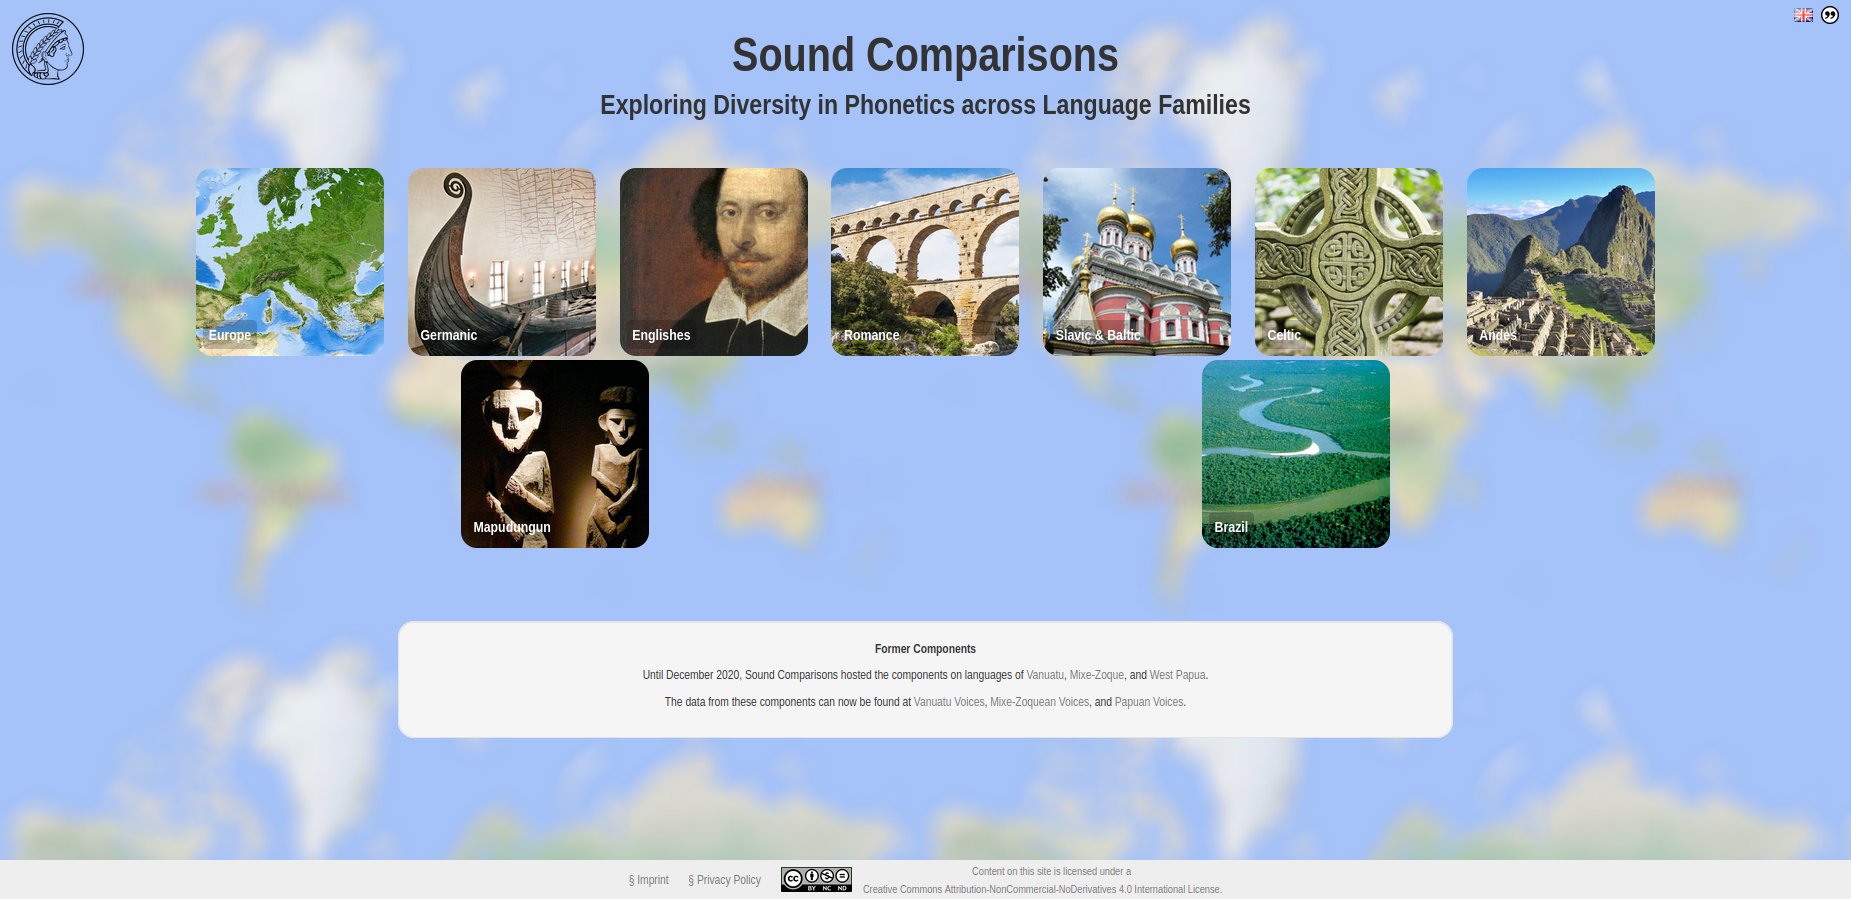
\includegraphics[width=1\linewidth]{substance/images/soundcompa1}
	\caption[Page d'accueil du site web de Sound Comparisons]{Page d'accueil du site web de Sound Comparisons : Les données du projet Sound Comparions pour chaque \textg{étude} sont accessibles sur internet via le site web disponible sur \url{https://soundcomparisons.com/\#home}.}
	\label{fig:soundcompa1}
\end{figure}

\begin{figure}
	\centering
	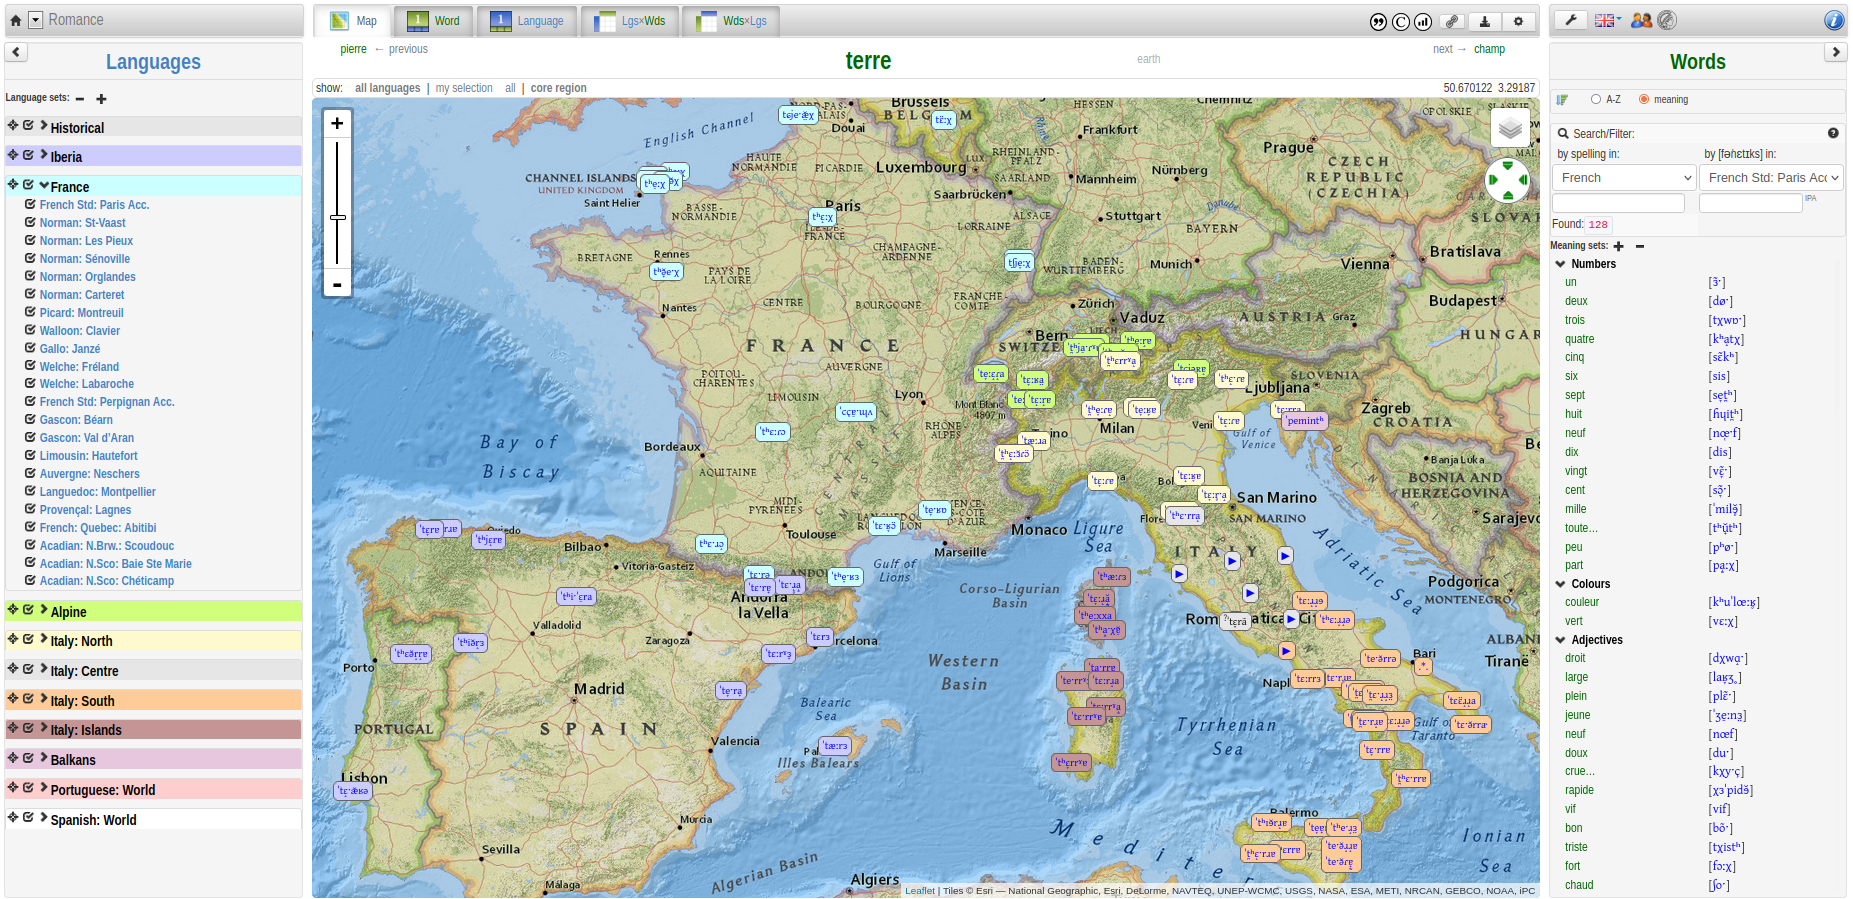
\includegraphics[width=1\linewidth]{substance/images/soundcompa2}
	\caption[Distribution des transcriptions du cognat \textsc{terre} dans les langues romanes]{Distribution des transcriptions du cognat \href{https://soundcomparisons.com/\#/en/Romance/map/earth/Lgs_Sln}{\textsc{terre}} dans les langues romanes. Pour chaque étude et chaque cognat, il est possible de visualiser la distribution géographique des transcriptions avec les audios associés.}
	\label{fig:soundcompa2}
\end{figure}

Différentes familles de langues et aires linguistiques sont représentées dans Sound Comparisons (dernier accès au 4/06/20):

\begin{itemize}
	\item Europe
	\item Germanic
	\item Englishes
	\item Romance (Figure \ref{fig:soundcompa2})
	\item Slavic
	\item Celtic
	\item Andes
	\item Mapudungun
	\item Brazil
	\item Vanuatu (hébergé depuis décembre 2020 sur \href{https://vanuatuvoices.clld.org/}{Vanuatu Voices}\footnote{Disponible sur : \url{https://vanuatuvoices.clld.org}})
	\item West Papua (hébergé depuis décembre 2020 sur \href{https://papuanvoices.clld.org/}{Papuan Voices}\footnote{Disponible sur : \url{https://papuanvoices.clld.org}})
	\item Mixe-Zoque (hébergé depuis décembre 2020 sur \href{https://mixezoqueanvoices.clld.org/}{Mixe-Zoquean Voices}\footnote{Disponible sur : \url{https://mixezoqueanvoices.clld.org}})
\end{itemize}

\section{Questions de recherche}

Plusieurs questions ont émergé sur la base de la multitude de données présentes dans Sound Comparisons, des enregistrements audios et des transcriptions plus ou moins étroites associées. \\

Premièrement, est-il possible de faire un inventaire, aussi exhaustif que possible, des symboles utilisés pour faire référence aux rhotiques ?
Nous considérons ici les rhotiques comme formant une classe phonologique et nous nous interrogeons sur ses membres, les unités phonétiques, qui la composent.

Deuxièmement, à quel point les transcriptions des rhotiques mettent en évidence de la variation ? Et, est-ce que cette variation, si elle est présente, se retrouve aussi dans les reconstructions de langues historiques ou de proto-langues ?
Il faut s'interroger sur ce que la variation signifie à la fois dans les transcriptions, mais aussi dans les rhotiques.\\

Finalement, quel segment ou quels segments sont les meilleurs exemplaires de cette classe ? 
Par meilleurs exemplaires, nous comprendrons ici les productions les plus fréquentes, les plus caractéristiques de la classe phonologique.\\

En ce qui concerne spécifiquement le trill et le tap, nous nous sommes aussi posé différentes questions sur la base des résultats obtenus dans les chapitres que nous avons développés précédemment. Quelle est la place du trill et du tap dans les transcriptions ? Est-ce que la représentation du tap est plus utilisée dans les transcriptions étroites que celle du trill ?\\

Sachant que Sound Comparisons se base sur l'étude de plusieurs variétés de langues appartenant à des familles de langues différentes qui ont été transcrites par différentes personnes, on peut se demander comment varie la description des rhotiques en fonction de la transcription. Pour cela, nous devons faire attention aux profils des personnes ayant transcrit les données.

\section{Étude de cas 1 : Le cas de \textg{3} en Europe}

Nous avons utilisé l'étude \textg{Europe} \parencite{heggarty_sound_2019-2} de Sound Comparisons pour notre première étude de cas dans le but de comprendre la structure des données.
Cela inclut les langues germaniques, romanes, balto-slaves et celtiques qui ont été transcrites dans Sound Comparisons \parencite{heggartySoundComparisonsNew2019}. Toutes sont des langues indo-européennes \glotto{indo1319}. \\

Pour cette première étude de cas, nous n'avons inclus qu'un seul cognat : \textg{3}. En effet, de tous les cognats dont la forme est partagée par les différents groupes de langues inclus et dans les transcriptions, il s'agit d'un des seuls possédant un son \textg{simil-\textit{r}}. Ce segment est généralement présent en attaque complexe initiale de mot.\\

Nous avons collecté au total 339 transcriptions pour 335 variétés langagières. Il s'agit de variétés principalement présentes en Europe mais aussi présentes au Canada pour des variétés de français canadien, au Brésil pour des variétés de portugais brésilien ou encore en Afrique du Sud pour l'afrikaans.

\subsection{Nettoyage des données}

Dans le but d'avoir des résultats plus simples et fiables à interpréter, nous avons fait le choix de ne pas travailler directement avec les données transcrites brutes mais de procéder à un nettoyage pour obtenir des transcriptions plus facilement analysables.
Pour cela, nous avons systématiquement supprimé tous les diacritiques présents dans les transcriptions. Ces diacritiques peuvent correspondre à un lieu d'articulation secondaire, le voisement ou encore l'accent. Bien que cela présente des avantages pour la simplicité de l'analyse, il faut être conscient que certains diacritiques permettent de faire la distinction entre certaines fricatives et leurs contreparties approximantes comme la fricative voisée uvulaire [ʁ] et l'approximante voisée uvulaire [ʁ̞], ou encore entre 
deux lieux d'articulation comme les dentales (spécifiées avec un diacritique) et les alvéolaires (sans diacritique). Par exemple, [r] est alvéolaire alors le trill dental [r̪] est obtenu en ajoutant un diacritique.\\ 

Nous nous sommes appuyé sur la liste de diacritiques disponibles dans le clavier API en ligne Lexilogos (\url{https://www.lexilogos.com/clavier/api.htm}, visité le 04/04/2020). Nous avons aussi ajouté à cette liste les symboles utilisés pour les frontières entre les syllabes qui sont généralement représentées par un point, et nous avons supprimé l'astérisque utilisé dans Sound Comparisons pour représenter les données manquantes.\\

Voici la liste de diacritiques, représentés avec le cercle en pointillé, et des autres symboles, à supprimer des données que nous avons récupérées :
{\fontspec{Charis SIL}  ˈ◌, ˌ◌, ◌ː, ◌ˑ, ◌ʼ, ◌ʴ, ◌ʰ, ◌ʱ, ◌ʲ, ʷ, ◌ˠ, ◌ˤ, ◌˞ , ◌̃, ◌̴ , ◌̊, ◌̆, ◌̈, ◌̽, ◌̚, ◌̋, ◌́, ◌̄, ◌̀, ◌̏, ◌̌, ◌̂, ◌̥, ◌̤, ◌̪, ◌̬, ◌̰, ◌̺, ◌̼, ◌̻, ◌̹, ◌̜, ◌̟, ◌̠, ◌̝, ◌̩, ◌̞, ◌̯, ◌̘, ◌̙, ., *}. Au delà de présenter uniquement la liste des diacritiques, cela montre l'étendue des possibilités des modificateurs de caractères API pour les transcripteurs/trices.\\

Nous avons aligné les phones présents dans les transcriptions après l'extraction des diacritiques. Nous avons basé notre analyse sur le caractère et non sur le segment (les segments complexes comme les affriquées sont considérés comme deux caractères). En moyenne, nous avons des mots pour le cognat \textg{3} de 3,7 caractères après nettoyage.

\subsection{Résultats des réalisations pour le cognat \textg{3}}

On peut s'intéresser à plusieurs positions dans le mot pour trouver la rhotique.
Par exemple, si on regarde en position initiale des mots du cognat \textg{3}, on retrouve les caractères suivants (on précisera à chaque fois comment le caractère est décrit par l'API et on donnera les possibilités principales de modification du caractère) :

\begin{itemize}
	\item la fricative non voisée dentale \textit{θ} (caractère qui peut aussi être partagé avec la fricative non-voisée labio-linguale \textit{θ̼})
	\item la fricative alvéolaire non voisée \textit{s} (caractère qui peut aussi être partagé avec les fricatives dentale \textit{s̪} et post-alvéolaire non-voisées \textit{s̠})
	\item l'occlusive alvéolaire non-voisée \textit{t} (caractère qui peut aussi être partagé avec ses contreparties labio-linguale \textit{t̼}, dentale \textit{t̪} et post-alvéolaire \textit{t̠})
	\item l'occlusive alvéolaire voisée \textit{d} (caractère qui peut aussi être partagé avec ses contreparties labio-linguale \textit{d̼}, dentale \textit{d̪} et post-alvéolaire \textit{d̠})
	\item l'occlusive rétroflexe non-voisée \textit{ʈ}
\end{itemize}

Nous ne considérons pas les différentes occlusives comme des rhotiques. Néanmoins, la présence de la rétroflexe \textit{ʈ} interroge. On la retrouve pour dix variétés langagières au sud de l'Italie et en Sicile.
Il a été postulé que l'émergence du \textit{ʈ} rétroflexe s'expliquerait par une assimilation régressive du lieu d'articulation de la rhotique, qui a subit un changement de son lieu d'articulation vers la rétroflexion (cf. \textcite[53--55]{celataAnalisiProcessiDi2006} pour une revue de la littérature sur la rétroflexion de la rhotique et de l'occlusive).\\

La position qui nous intéresse pour chercher les segments consonantiques \textg{simil-r} est celle après l'occlusive initiale. Le choix du cognat \textg{3} se justifie car il est généralement réalisé avec peu de phones, et on retrouve souvent une attaque branchante contenant la rhotique, c'est-à-dire, dans un groupe consonantique où la deuxième consonne est une rhotique précédant une voyelle.
On y retrouve : 

\begin{itemize}
	\item \textit{r} : le trill alvéolaire voisé (caractère qui peut aussi être partagé par les lieux d'articulation labio-lingual, dental, alvéolaire et post-alvéolaire voisés et non voisés). Dans les données de Sound Comparisons, cela correspond à 5 segments: [r], [r̴], [rˠ], [r̝] et [r̥ʲ]
	\item \textit{ɹ} : l'approximante alvéolaire voisée (caractère qui peut aussi être partagé par les lieux d'articulation labio-lingual et alvéolaire voisés et non voisés). Dans les données cela correspond à 3 segments différents : [ɹ], [ɹ̥] et [ɹ̥ʲ]
	\item \textit{χ} : la fricative uvulaire voisée. Dans les données cela ne correspond qu'à un segment : [χ]
	\item \textit{ɾ} : le tap ou flap alvéolaire voisé (caractère qui peut aussi être non voisé). Dans les données cela correspond à 6 segments différents : [ɾ], [ɾˠ], [ɾ̥], [ɾʲ], [\fontspec{Charis SIL}ɾ̝̥\fontspec{Linux Libertine O}] et [ɾ̝]
	\item \textit{ʁ} : la fricative uvulaire voisée (caractère aussi partagé avec l'approximante uvulaire voisée). Dans les données cela correspond à 3 segments : [ʁ], [ʁ̞] et [ʁ̥]
	\item \textit{ɻ}~~ : l'approximante rétroflexe (voisée et non-voisée). Dans les données cela ne correspond qu'à 1 segment : [ɻ]
	\item \textit{x} : la fricative vélaire non-voisée. Dans les données cela correspond à 2 segments différents : [x] et [x̠]
	\item \textit{ɽ} : le flap rétroflexe (voisé et non-voisé). Dans les données cela correspond à : [ɽ]
	\item \textit{s} : la fricative alvéolaire non-voisée. Dans les données cela correspond vraisemblablement à une affriquée : [ts]
	\item \textit{ʂ} : la fricative rétroflexe non voisée. Dans les données cela correspond vraisemblablement, dans certains cas, à une affriquée : [ʈʂ] ou à [ʂ]
	\item \textit{ɕ} : la fricative alvéo-palatale. Dans les données cela correspond à : [ɕ] et [ɕ̝]
	\item \textit{w} : l'approximante labio-vélaire. Dans les données cela correspond à : [w]
	\item \textit{j} : l'approximante labio-vélaire. Dans les données cela correspond à : [j]
\end{itemize}

Dans certains cas, où la rhotique n'était pas dans les deux premiers segments du mot, nous avons dû regarder le troisième caractère. Dans ces cas, on retrouve les segments suivants : 

\begin{itemize}
	\item \textit{r} : le trill, présent dans les données après un schwa épenthétique [ə]
	\item \textit{ɾ} : le tap ou flap, présent dans les données après une voyelle épenthétique [ə] ou [ɵ]
	\item {ɻ}: l'approximante rétroflexe, toujours présente après [ʈʂ]
	\item \textit{ʂ} : la fricative rétroflexe non-voisée, présente dans les données après [tʂ]
\end{itemize}

Au total, nous avons compté 28 segments différents qui pouvaient être inclus comme des segments \textg{simil-r} dans les groupes de langues parlées en Europe pour le cognat \textg{3} que nous avons décidé de représenter sous la forme d'un graphe pour faciliter la visualisation de la multitude de symboles pouvant être utilisés pour transcrire ce qui généralement sera transcrit orthographiquement avec un <r>.\\

\begin{figure}
	\centering
	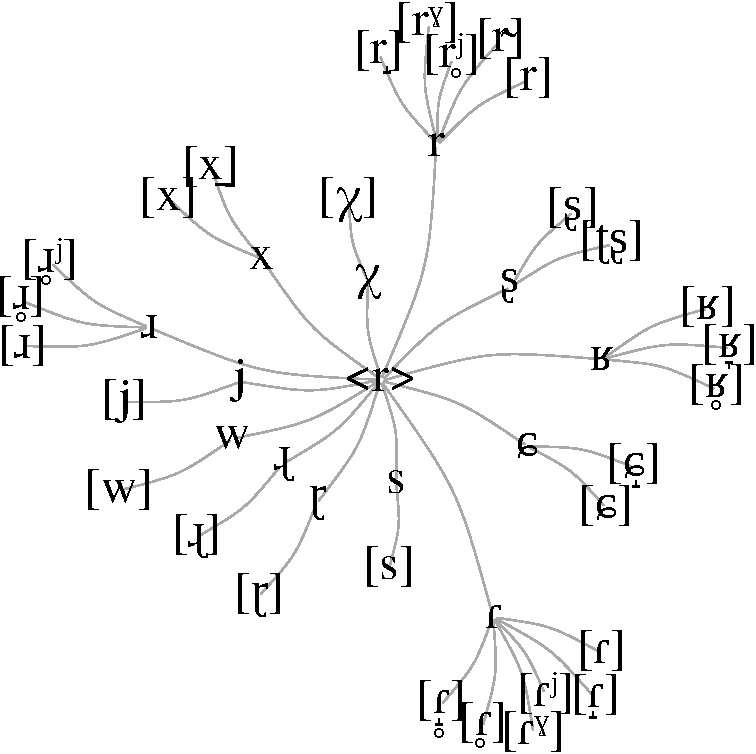
\includegraphics[width=0.7\linewidth]{substance/images/europe_three1CROP}
	\caption[Graphe des différentes réalisations de la rhotique dans les variétés d'Europe]{Graphe des différentes réalisations de la rhotique dans les variétés d'Europe à partir des données de Sound Comparisons. Au centre du graphe on retrouve le graphème <r> rattaché à différents segments \textg{nus} sans diacritiques, utilisés comme niveau intermédiaire pour l'analyse. À ces segments sont rattachées les transcriptions étroites des rhotiques. Le graphe est obtenu avec le package \texttt{igraph} \parencite{csardiIgraphSoftwarePackage2006}.}
	\label{fig:europethree}
\end{figure}

Ces 28 segments sont représentés dans la figure \ref{fig:europethree} où l'on retrouve les symboles associés aux différentes réalisations de la rhotique qui, dans la majorité des cas, sont en attaque branchante dans le cognat \textg{3} dans l'étude de Sound Comparisons \textg{Europe}. Au centre du graphe se trouve le graphème <r> (une simplification de la représentation orthographique du \textit{r}) qui est rattaché à différents caractères sans diacritiques. Ces caractères \textg{nus} représentent un niveau intermédiaire d'analyse, ils peuvent capturer certains des traits des segments comme la manière d'articulation et le lieu d'articulation. Les segments, issus des transcriptions des rhotiques se situent au niveau des nœuds terminaux et sont directement rattachés aux caractères intermédiaires.\\

\begin{figure}
	\centering
	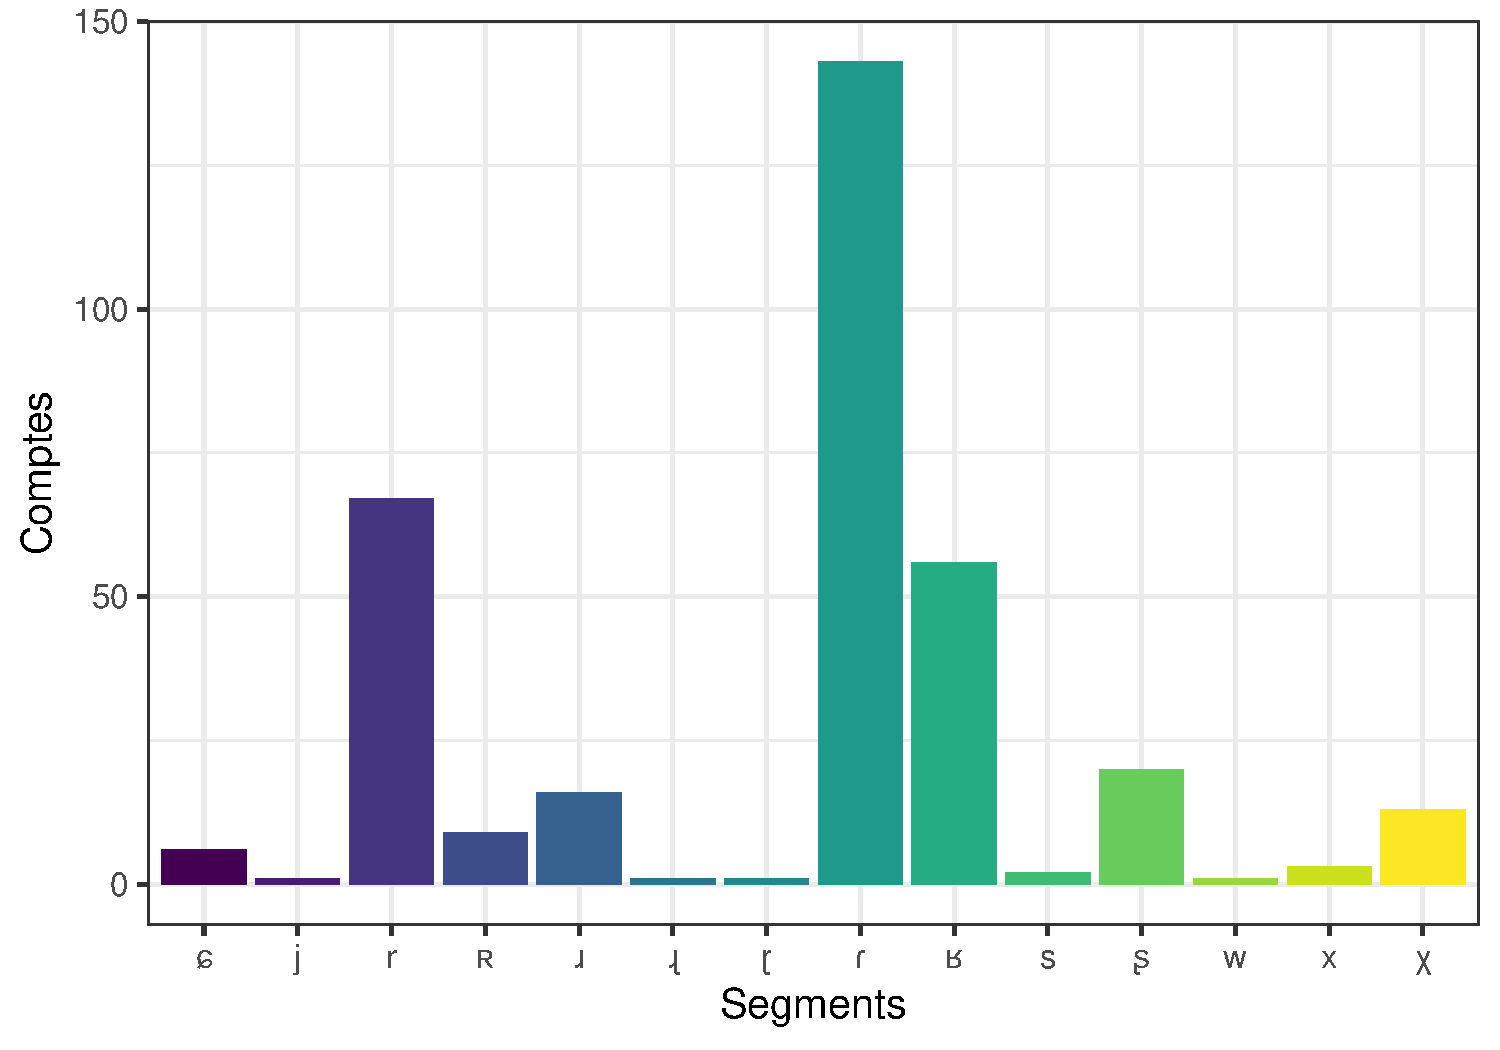
\includegraphics[width=1\linewidth]{substance/images/counts_1_europe}
	\caption[Comptes des différents segments pour le cognat \textg{3} dans les langues d'Europe]{Comptes des différents segments pour le cognat \textg{3} dans les langues d'Europe.}
	\label{fig:counts1europe}
\end{figure}

Ces segments ne sont pas présents dans les mêmes proportions. Si l'on compte les occurrences de chaque caractère apparaissant dans notre niveau intermédiaire d'analyse, on obtient des différences entre les caractères. En Figure \ref{fig:counts1europe}, on observe que \textit{ɾ} est le plus fréquent (n = 143 soit 42\% des productions), suivi par \textit{r} (n = 67 soit 20\% des productions) et \textit{ʁ} (n= 56 soit 17\% des productions). Les réalisations antérieures sont plus fréquentes que les réalisations postérieures (n = 251 soit 74\% contre n = 88 soit 26\% des productions). Cependant, il faut prendre en compte que la taille de l'échantillon dont nous disposons peut influencer les résultats en favorisant certaines variétés.\\

L'étude de la rhotique sur le cognat \textg{3} dans les langues d'Europe, met en évidence que :
\begin{enumerate}
	\item Toutes les variétés ne produisent logiquement pas le /r/ de la même manière
	\item La catégorie du tap ou flap [\fontspec{Charis SIL} \small ɾ ɾˠ ɾ̥ ɾʲ ɾ̝̥  ɾ̝\fontspec{Linux Libertine O}\normalsize] représentée par le \textit{ɾ} correspond à la catégorie d'allophone la plus fréquente, suivie par celle du trill alvéolaire [r r̴ rˠ r̝  r̥ʲ] représentée par le \textit{r}
	\item Certaines variétés ont des productions antérieures (avec des consonnes dentale, alvéolaire ou rétroflexe), et d'autres postérieures (avec des consonnes vélaire, uvulaire ou glottale)
\end{enumerate}

Nous soulignons le fait que certaines transcriptions ont été décrites comme étroites. C'est le cas des transcriptions des variétés de l'étude \textg{anglais}, \textg{romane} et \textg{balto-slave}. D'autres transcriptions sont décrites comme plus larges. C'est le cas pour les variétés \textg{germaniques}.\\
C'est pourquoi notre deuxième étude de cas sur Sound Comparisons portera sur les deux études de Sound Comparisons où les transcriptions sont décrites comme étroites (les études \textg{romane} et \textg{slave}) que nous comparerons avec une étude plus large (l'étude \textg{germanique}) dans notre troisième étude de cas. Enfin, nous conclurons sur le cas du mapudungun, une langue d'Amérique du sud, où les transcriptions sont aussi étroites.

\section{Étude de cas 2 : le cas des langues slaves et romanes}

Dans cette deuxième étude de cas, nous avons pris en compte les transcriptions des langues slaves et des langues romanes.

\subsection{Description des langues romanes}

Le groupe des langues romanes se compose de 105 variétés langagières et du latin classique. Nous avons selectionné 43 cognats sur la base de la présence de <r> dans les mots reconstruits par le projet Sound Comparisons. Les transcriptions ont été faites par \href{https://unina.academia.edu/GiovanniAbete}{Giovanni Abete}, un linguiste italien qui s'intéresse à l'étude des dialectes des langues romanes et plus particulièrement des dialectes de l'Italie. Sa \href{https://www.academia.edu/2362845/I_processi_di_dittongazione_nei_dialetti_dell_Italia_meridionale_Un_approccio_sperimentale}{thèse} \parencite{abeteProcessiDiDittongazione2010} écrite en italien porte sur les processus de diphtongaison dans les dialectes de l'Italie du sud.\\

Parmi les variétés langagières des langues romanes\footnote{Il ne s'agit pas d'une liste exhaustive et on y associe des références d'\textit{Illustrations of the IPA} ou d'études mentionnant la variation dans les rhotiques.} on trouve le galicien \parencite{regueiraGalician1996}, l'asturien \parencite{muniz-cachonAsturian2018}, le portugais \parencite{cruz-ferreiraEuropeanPortuguese1995}, l'espagnol \parencite{haroEasternAndalusianSpanish2020}, le catalan \parencite{carbonellCatalan1992}, le français standard de Paris et de Perpignan \parencite{fougeronFrench1993}, le wallon, le normand \parencite{buscailFrenchOrneSpeaker2016}, le picard \parencite{prematRouleFrancaisDans2018}, le gascon \parencite{mooneyBearnaisGascon2014}, le francoprovençal \parencite{kasstanLyonnaisFrancoprovencal2015}, le romanche, le ladin \parencite{yangLadinVarietiesVal2021}, l'italien standard de Naples, de Rome ainsi que l'italien parlé dans plusieurs régions d'Italie \parencite{rogersItalian2004, bertinettoSoundPatternStandard2005}, le sarde \parencite{mereuCagliariSardinian2019} et le roumain \parencite{raduConditionedVariabilityRealization2016}. On retrouve des variétés de langues romanes, non parlées en Europe, comme avec le portugais du Brésil \parencite{barbosaBrazilianPortuguese2004} et du Mozambique, l'espagnol d'Amérique du Sud \parencite{avelinoMexicoCitySpanish2018,colomaArgentineSpanish2018} ou encore le français du Canada \parencite{sankoffLanguageChangeLifespan2007,sankoffInstabilityAlternationMontreal2013}.\\

Les variétés romanes sont généralement caractérisées par deux phonèmes rhotiques : le trill et le tap (on retrouve aussi parfois la mention du flap). Pour certaines variétés du portugais, une rhotique antérieure (généralement alvéolaire) s'oppose à une rhotique postérieure (généralement vélaire ou uvulaire). La rhotique uvulaire se retrouve aussi dans les variétés parlées en France où le contraste entre deux rhotiques a été perdu.
Le ladin et l'italien sont décrits comme ayant un seul trill. En ladin, ce trill est généralement réalisé comme un tap sauf dans la parole soignée. En italien, \textcite{rogersItalian2004} considèrent que l'allophone \textg{non marqué} est le [r]. \textcite{bertinettoSoundPatternStandard2005} n'emploient pas le terme de tap ou de flap pour parler de l'allophone à un battement mais mentionnent un contraste entre une rhotique simple et une rhotique géminée.

\subsection{Description des langues slaves}

Le groupe des langues slaves se compose de 28 variétés langagières. Nous avons sélectionné 39 cognats selon les mêmes critères que pour les langues romanes. Les transcriptions ont été faites par \href{https://orcid.org/0000-0002-4714-8462}{Lechosław Jocz}, un linguiste polonais qui s'intéresse à la dialectologie et aux langues slaves. Sa \href{https://www.academia.edu/7302143/Jocz_Wokalowy_system_hornjoserbskeje_r\%C4\%9B\%C4\%8De_p\%C5\%99itomnos\%C4\%87e}{thèse} \parencite{joczWokalowySystemHornjoserbskeje2011} écrite en polonais porte sur le système vocalique du haut sorabe.\\

De même que pour les langues romanes, on trouve une grande variété de langues slaves bien qu'elles soient moins nombreuses. On rencontre le letton \parencite{brenzingerNotesPhoneticsLatvian1973}, l'ukrainien \parencite{pompino-marschallUkrainian2017}, le biélorusse \parencite{birdBelarusian2020}, le russe \parencite{yanushevskayaRussian2015}, le rusyn, le polonais \parencite{jassemPolish2003}, le haut et bas sorabe \parencite{howsonUpperSorbian2017}, le tchèque \parencite{dankovicovaCzech1997,simackovaCzechSpokenBohemia2012}, le slovaque \parencite{hanulikovaSlovak2010}, le slovène \parencite{sustarsicSlovene1995}, le croate \parencite{landauCroatian1995}, le bosnien, le serbe, le macédonien ou encore le bulgare \parencite{ternesBulgarian1990}.\\

Ces différentes variétés slaves ont principalement été décrites comme ayant un \textg{trill}.
Le slovène est décrit avec un \textg{tap}, et le polonais comme ayant un segment \textg{flap/trill}.
Il est possible qu'un trill palatalisé soit présent en addition au trill, comme c'est le cas en ukrainien, en russe et en sorabe où la rhotique est uvulaire. \textcite{howsonUpperSorbian2017} mentionne un \textg{hard} et un \textg{soft} trill uvulaire. \textcite{zygisMarkednessTrillsCase2004} montre dans son tableau (12) (p. 151) que les langues slaves ont toutes hérité d'un trill (même le slovène), et que le bulgare ainsi que les langues précédemment mentionnées ont un trill palatalisé dont la distribution dans la syllabe est plus ou moins restreinte.
Les auteurs des \textit{Illustrations of the IPA} des langues slaves s'accordent pour dire que le trill palatalisé est généralement réalisé comme un tap. De même, pour le slovaque, où la rhotique existe dans une version géminée (mais sans paire minimale pour postuler deux phonèmes), la rhotique non-géminée est généralement réalisée comme un tap.

\subsection{Résultats des caractérisations de la rhotique dans les langues romanes et slaves}

Avant d'exposer les résultats des deux études, afin de situer les transcriptions que nous avons analysées, il nous parait important de dire que les transcripteurs de chaque étude ont le point commun d'avoir principalement travaillé pendant leur thèse sur des segments vocaliques en y incluant des analyses acoustiques. Ces deux chercheurs sont intéressés par la dialectologie, et donc par l'étude de la variation.\\

En se basant sur la même méthodologie que pour l'étude \textg{Europe}, on obtient des graphes pour les variétés romanes et les variétés slaves avec des niveaux intermédiaires d'analyse et les nœuds terminaux pour les réalisations phonétiques possibles.\\

\begin{figure}
	\centering
	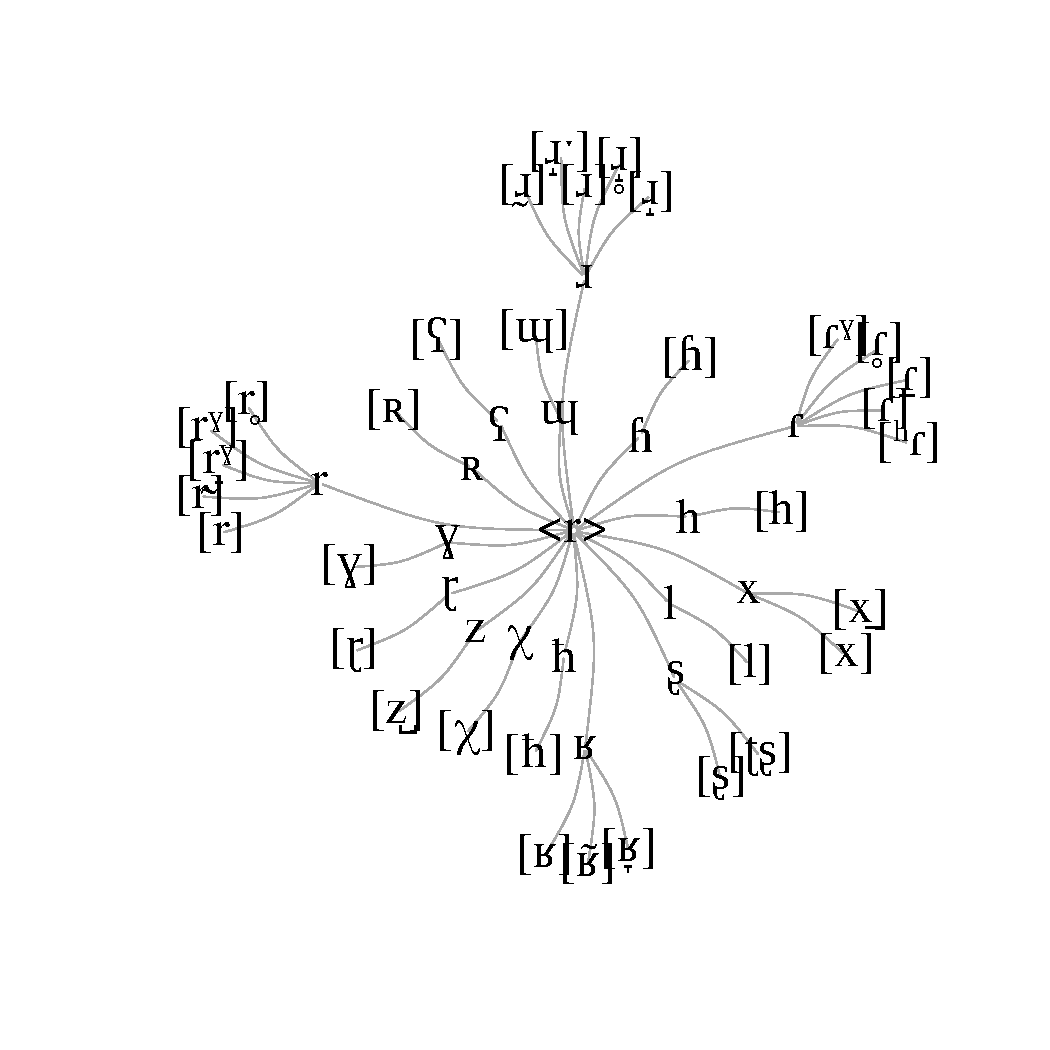
\includegraphics[width=\linewidth]{substance/images/romance_rhotics}
	\caption[Graphe des différentes réalisations de la rhotique dans les variétés romanes]{Graphe des différentes réalisations de la rhotique dans les variétés romanes à partir des données de Sound Comparisons. Nous représentons uniquement les réalisations de la rhotique quand elle est en position initiale ou en deuxième position d'attaque branchante. Le graphe est obtenu avec le package \texttt{igraph} (\texttt{v1.2.6}; Casardi \& Nepusz, 2006).}
	\label{fig:romancerhotics}
\end{figure}

Dans la figure \ref{fig:romancerhotics}, 17 caractères forment le niveau d'analyse intermédiaire dans les langues romanes. Au total, il y a 33 réalisations possibles pour les différents cognats pris en compte.
Six lieux d'articulations sont possibles avec les rhotiques alvéolaire, rétroflexe, vélaire, uvulaire et glottale, pour cinq manières d'articulation avec les trills, les taps, les flaps, les fricatives et les approximantes.
En moyenne chaque caractère intermédiaire possède environ 1,94 réalisations.\\

\begin{figure}
	\centering
	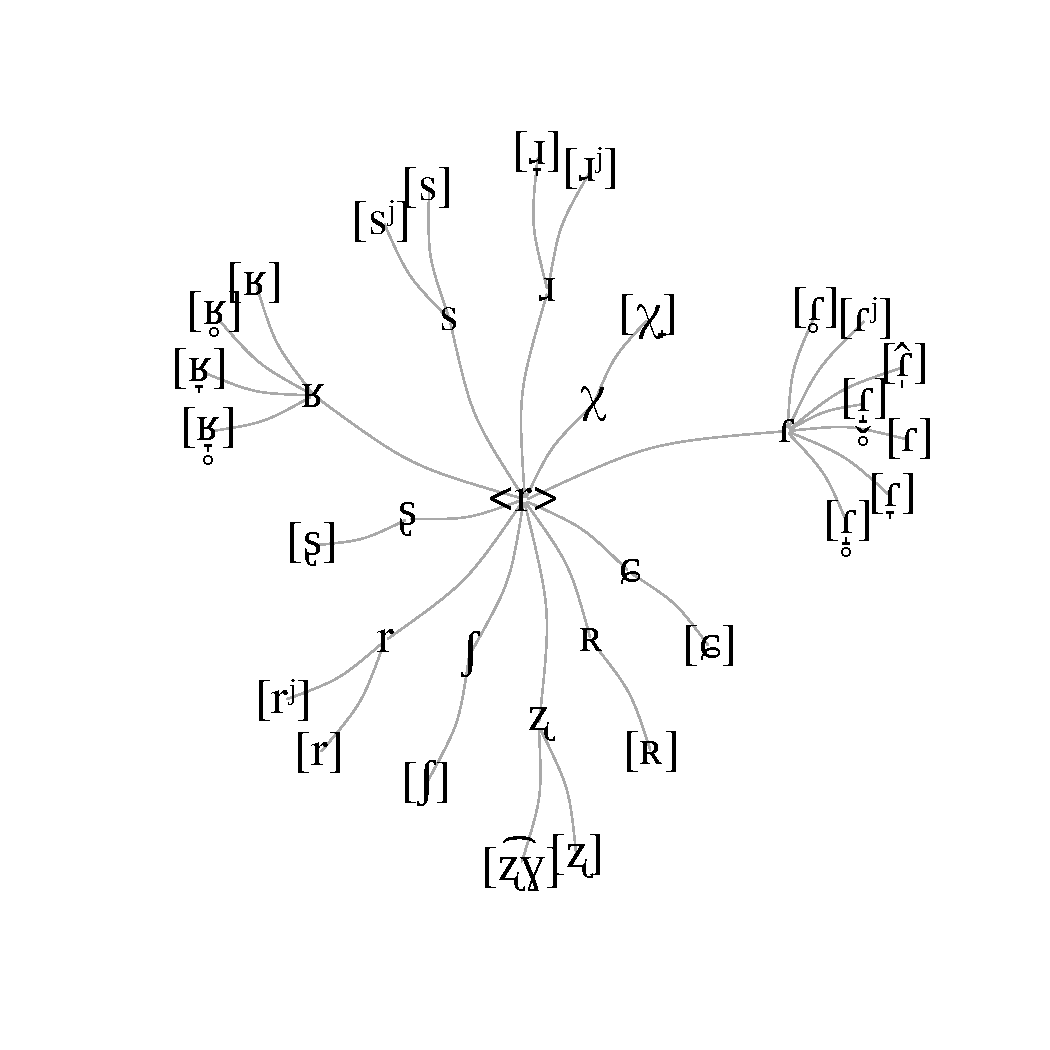
\includegraphics[width=\linewidth]{substance/images/slavic_rhotics}
	\caption[Graphe des différentes réalisations de la rhotique dans les variétés slaves]{Graphe des différentes réalisations de la rhotique dans les variétés slaves à partir des données de Sound Comparisons. Nous représentons uniquement les réalisations de la rhotique quand elle est en position initiale ou en deuxième position d'attaque branchante. Le graphe est obtenu avec le package \texttt{igraph} (\texttt{v1.2.6}; Casardi \& Nepusz, 2006).}
	\label{fig:slavicrhotics}
\end{figure}

Dans la figure \ref{fig:slavicrhotics}, 11 caractères forment le niveau d'analyse intermédiaire dans les langues slaves. Au total, il y a 24 réalisations possibles pour les différents cognats pris en compte.
On retrouve des rhotiques avec trois lieux d'articulations possibles : alvéolaire, rétroflexe et uvulaire, pour quatre manières d'articulation : trill, tap,  fricative et approximante.
En moyenne chaque caractère intermédiaire possède environ 2,18 réalisations.\\

\begin{figure}
	\centering
	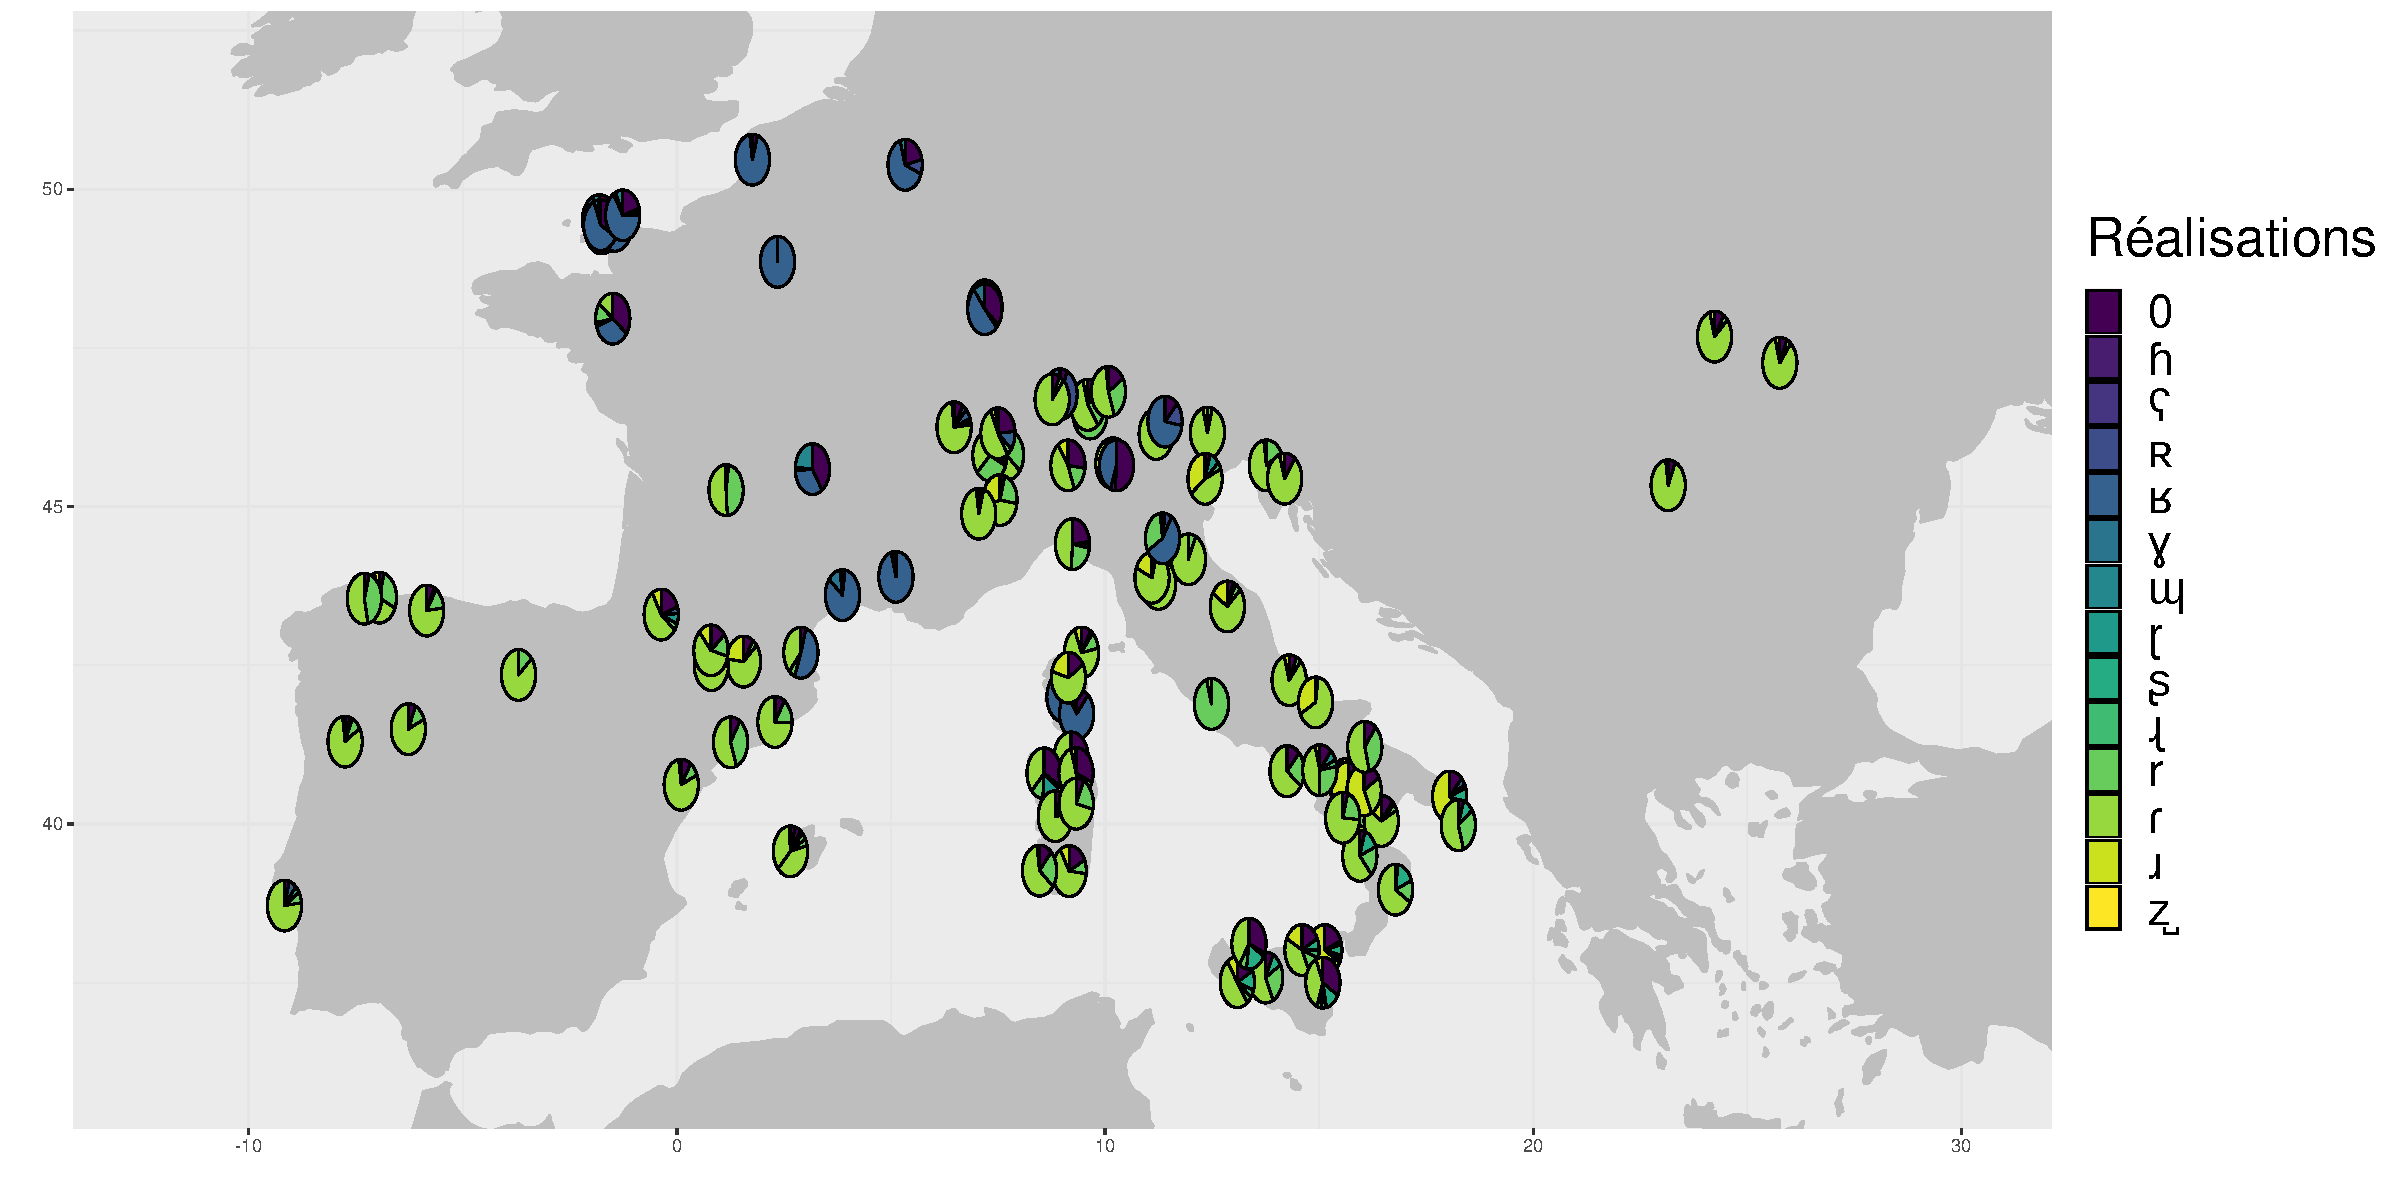
\includegraphics[width=1\linewidth]{substance/images/productionromane_1_viridis}
	\caption[Distribution des différentes réalisations dans les variétés romanes étudiées]{Distribution des différentes réalisations dans les variétés romanes étudiées. La carte montre seulement les variétés parlées en Europe continentale.}
	\label{fig:productionromane1viridis}
\end{figure}

Il est possible de visualiser dans un premier temps la diversité des réalisations pour les variétés romanes en Figure \ref{fig:productionromane1viridis}.
Tous les mots dans les variétés ne contiennent pas forcément une rhotique consonantique, nous avons donc codé son absence avec le \textit{0} (non présent dans la Figure \ref{fig:romancerhotics}). Cette absence peut s'expliquer soit par l'élision du segment, soit par la présence d'un segment vocalique non pris en compte par l'analyse.
On trouve principalement les allophones reliés aux \textit{ʀ ʁ χ} en France hexagonale et en Belgique, mais aussi en Corse, en Suisse et en Italie. 
On note la présence des fricatives pharyngale et glottale reliées à \textit{ħ ɦ h} qui ne sont pas présentes sur la carte. Ces allophones ont été produits dans les variétés portugaises du Brésil \parencite{rennickeVariationChangeRhotics2015}. Autrement, la présence du \textit{ɾ} semble majoritaire.\\

\begin{figure}
	\centering,
	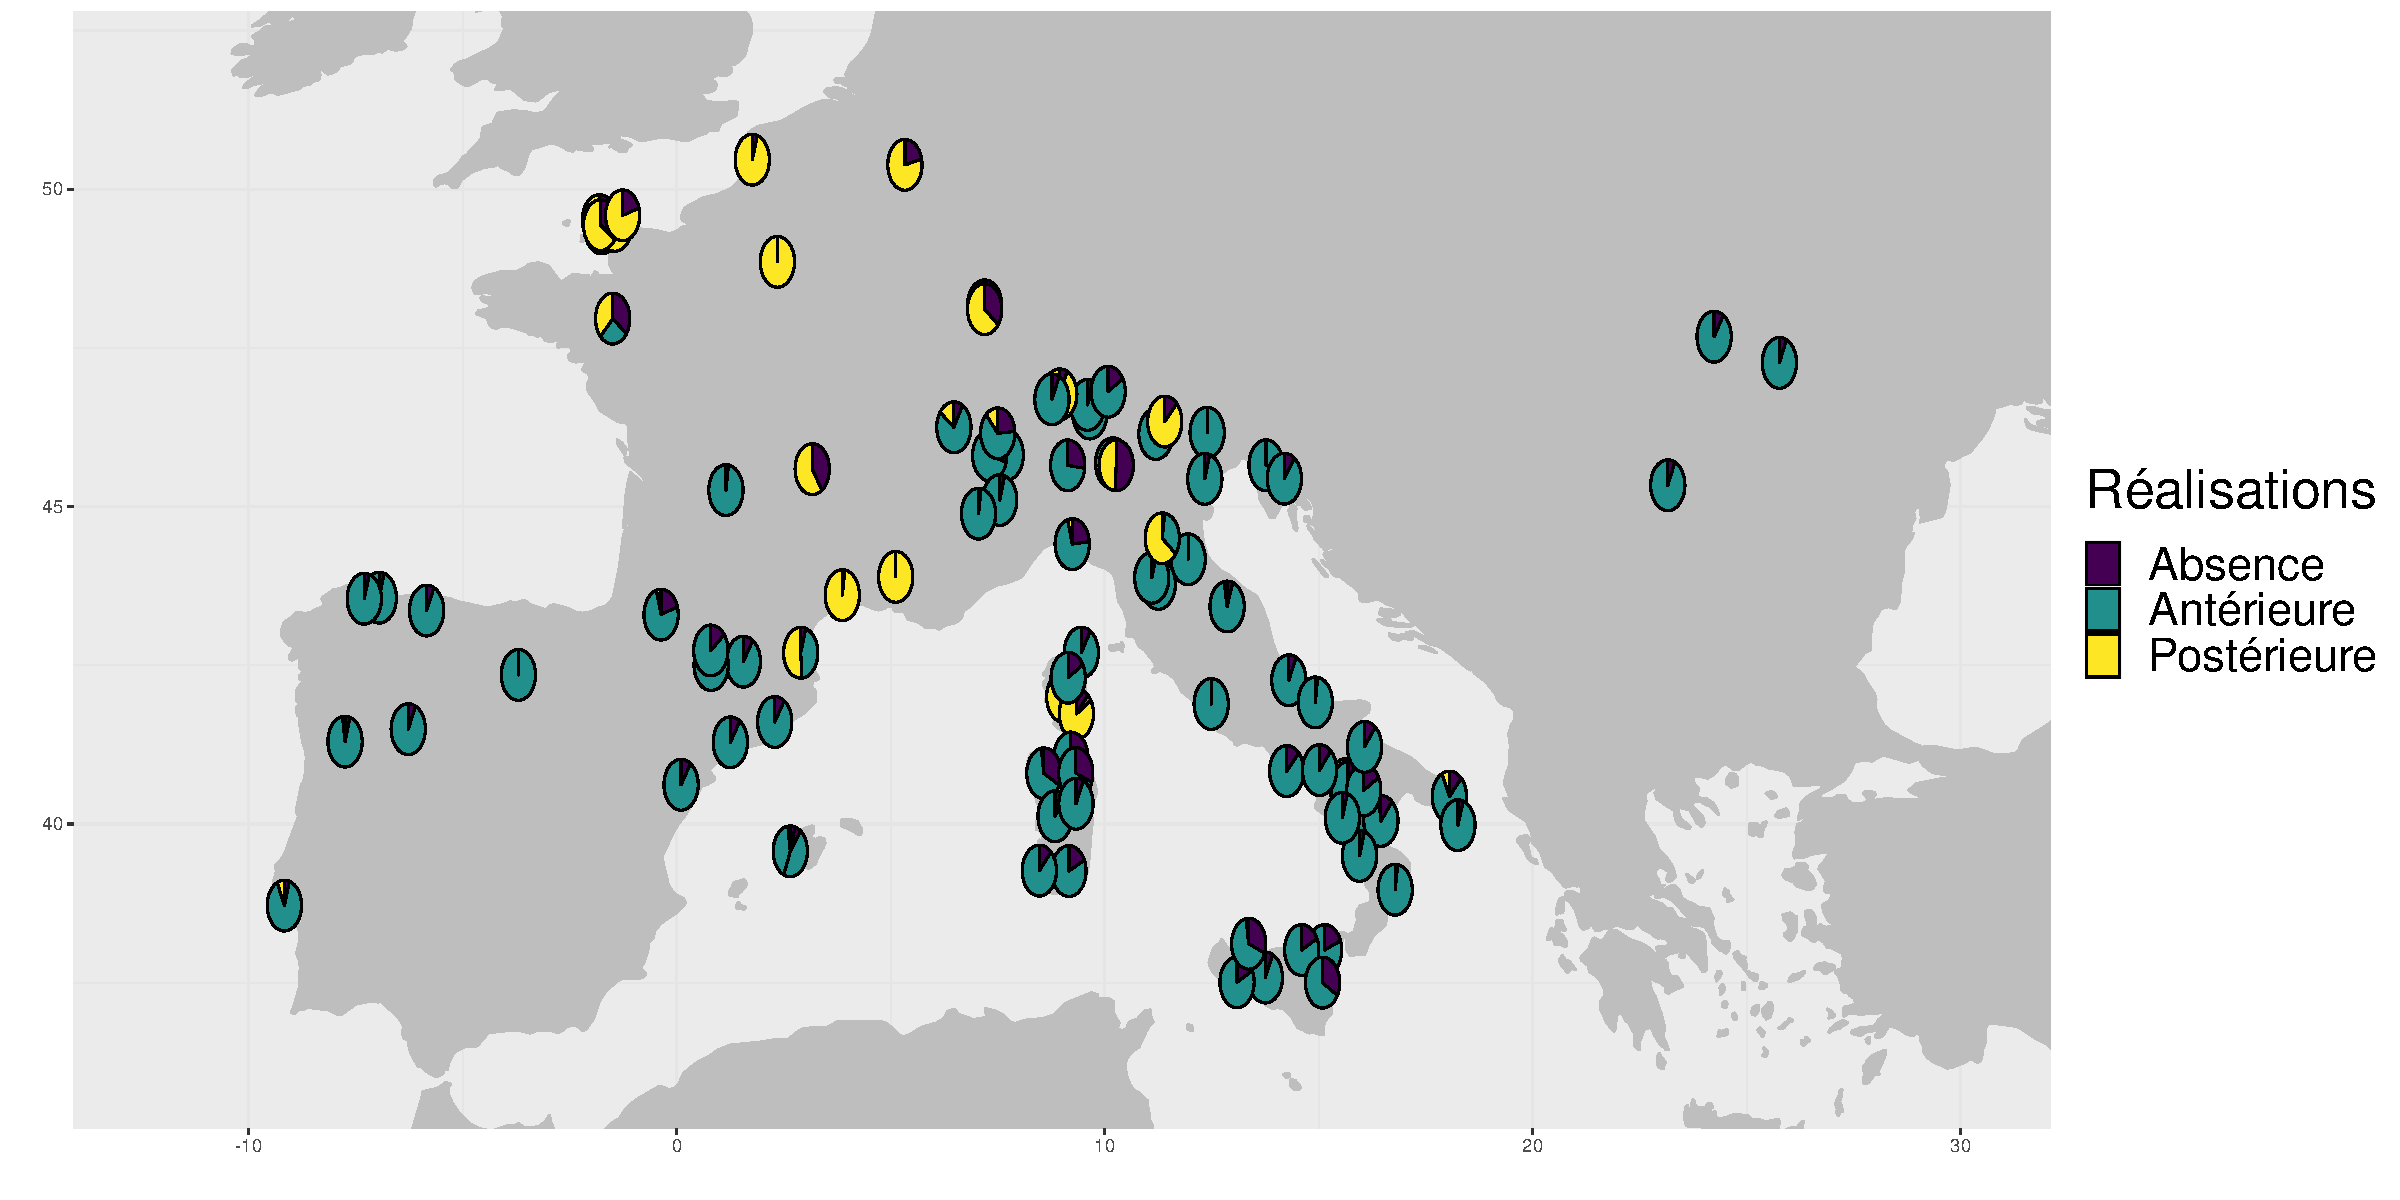
\includegraphics[width=1\linewidth]{substance/images/productionromane_2_viridis}
	\caption[Distribution des différentes réalisations dans les variétés romanes pour les productions antérieures et postérieures]{Distribution des différentes réalisations dans les variétés romanes étudiées en ne s'intéressant qu'à la dichotomie entre les productions antérieures et celles postérieures (et l'absence de segment).}
	\label{fig:productionromane2viridis}
\end{figure}

La figure \ref{fig:productionromane2viridis} permet de confirmer une différence au sein des langues romanes entre celles qui utilisent un lieu d'articulation antérieur pour la rhotique, comme c'est le cas de l'espagnol ou de l'italien, et celles qui utilisent un lieu d'articulation postérieur comme c'est le cas pour le français.\\

\begin{figure}
	\centering
	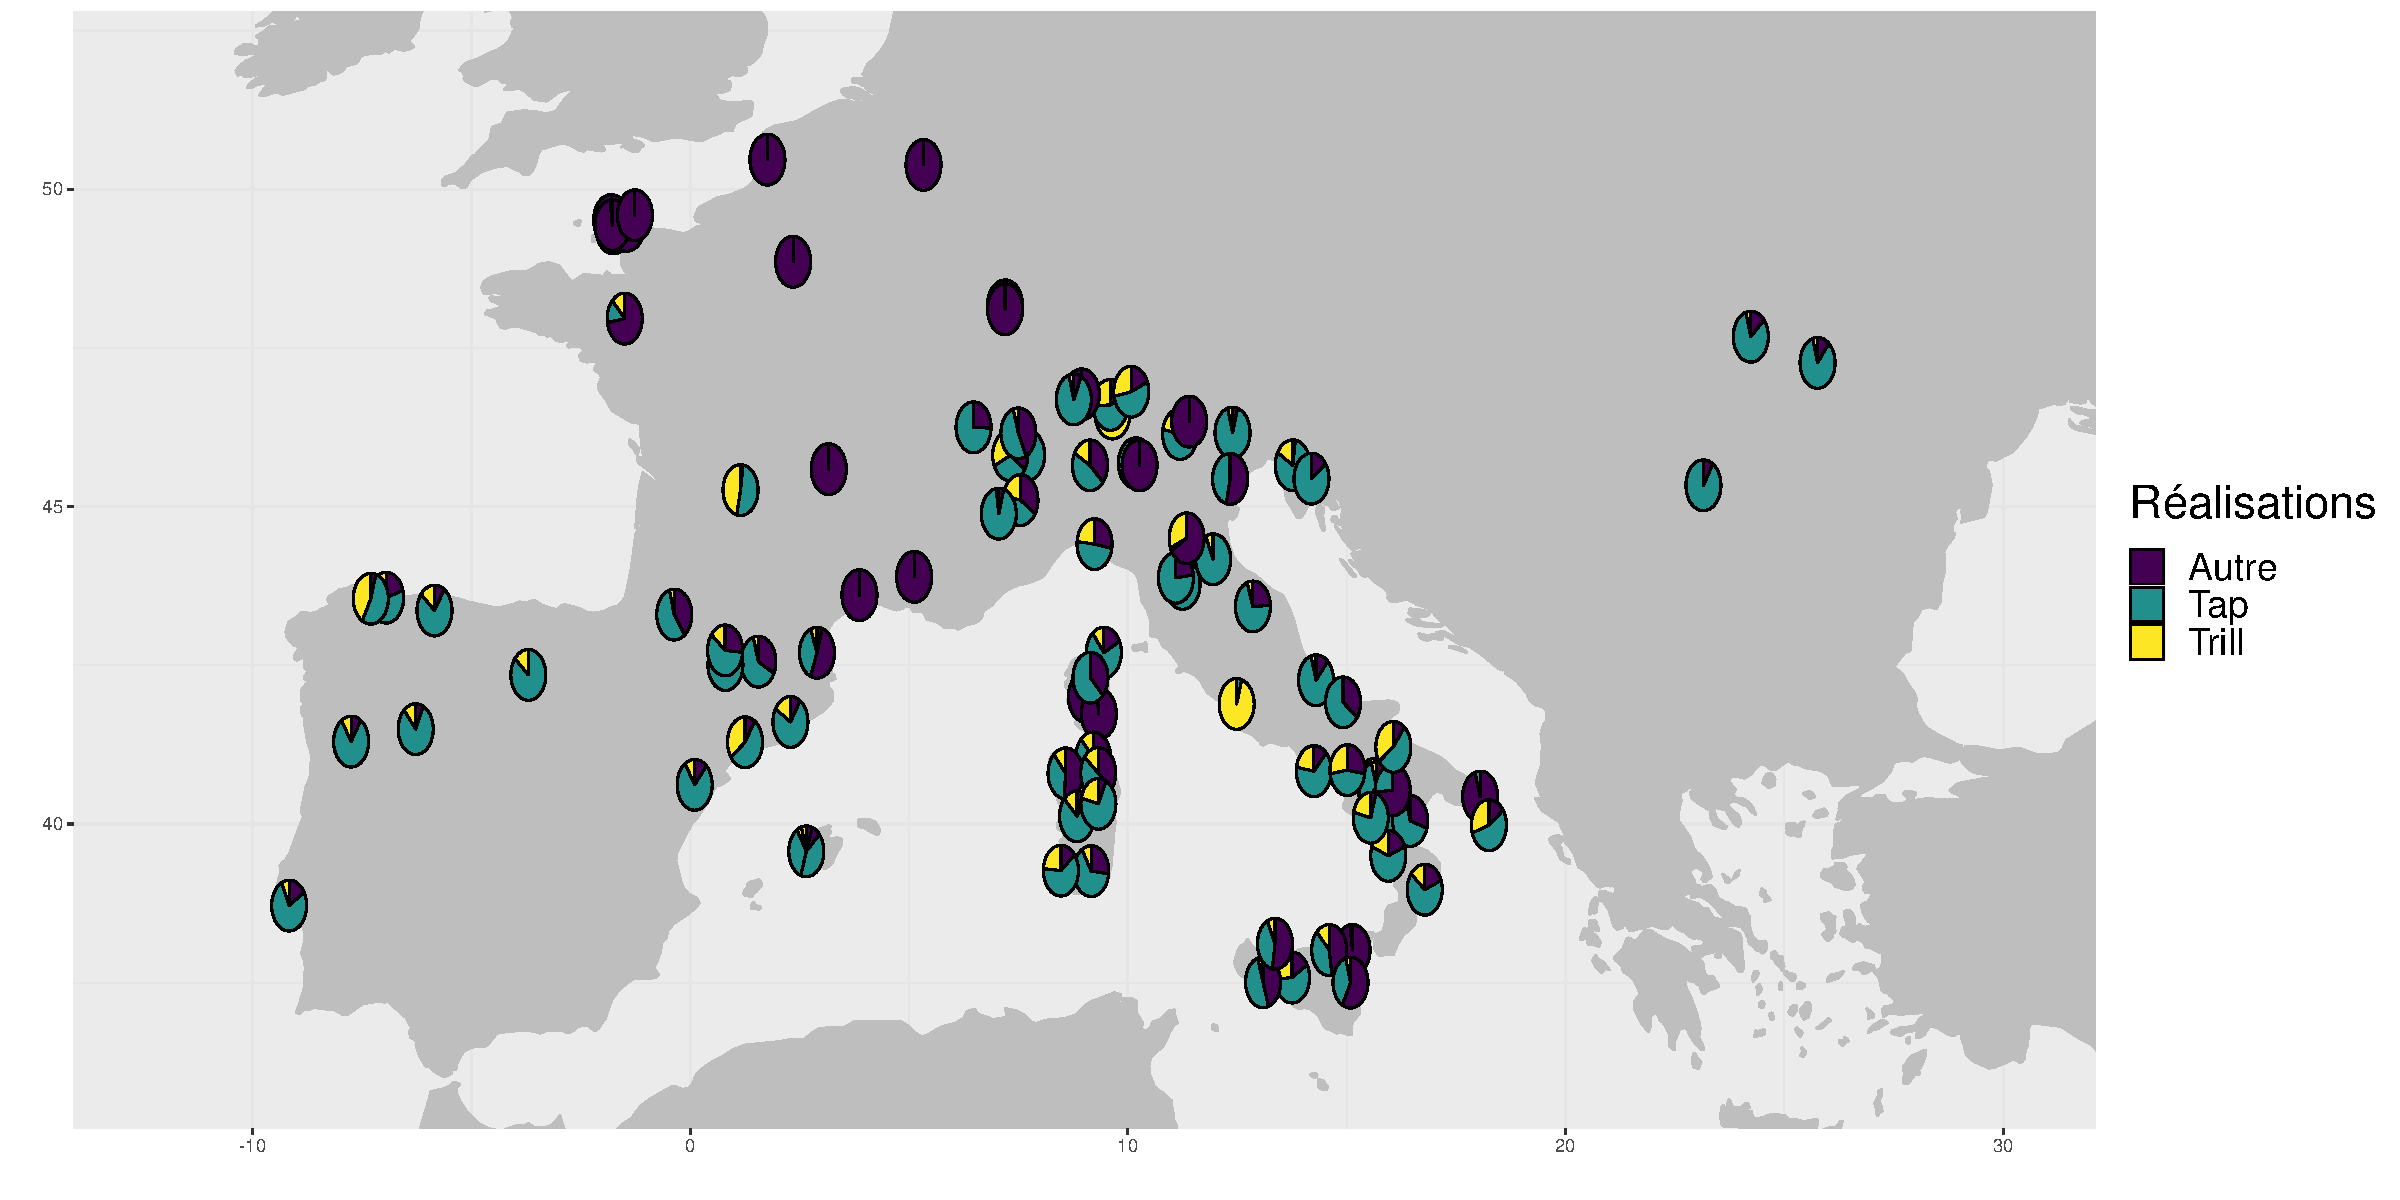
\includegraphics[width=1\linewidth]{substance/images/productionromane_3_viridis}
	\caption[Distribution des différentes réalisations dans les variétés romanes pour le trill et le tap]{Distribution des différentes réalisations dans les variétés romanes étudiées en ne s'intéressant qu'à la dichotomie entre trill et tap (et les autres segments).}
	\label{fig:productionromane3viridis}
\end{figure}

Lorsqu'on s'intéresse spécifiquement au trill et au tap, on observe en figure \ref{fig:productionromane3viridis} que le trill n'est jamais l'allophone majoritaire (à l'exception du latin classique, et nous reviendrons plus tard sur ce point). L'allophone majoritaire est le tap. On observe qu'il existe des variétés où on a un tap comme allophone mais pas de trill, le contraire n'existe pas. Il n'y a pas de variétés avec un trill mais sans tap.\\

\begin{figure}
	\centering
	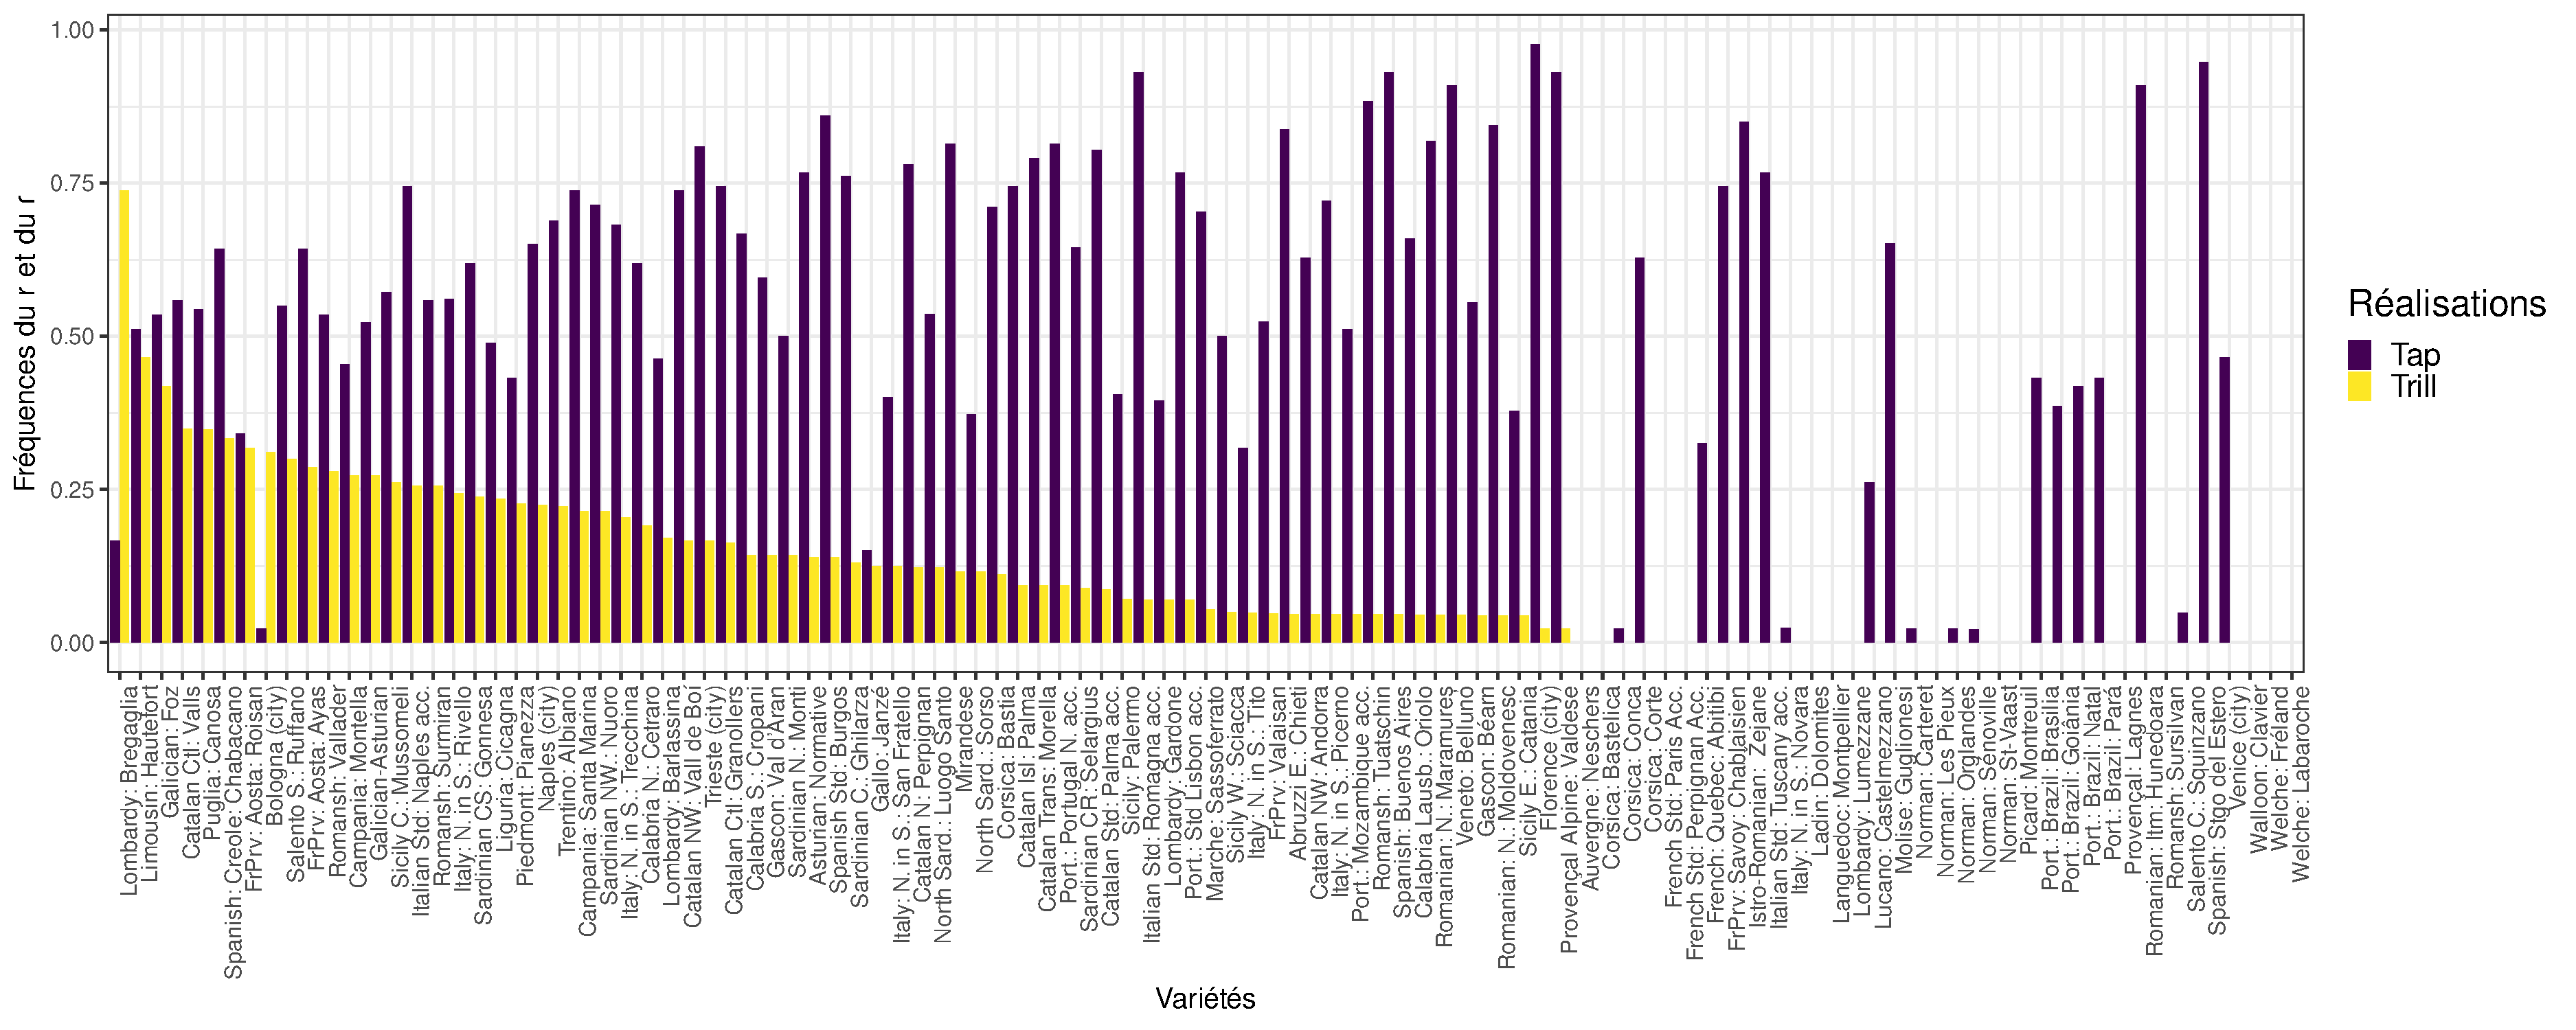
\includegraphics[width=1\linewidth]{substance/images/freq_trill_romance2}
	\caption[Fréquences du trill et du tap dans les variétés romanes]{Fréquences du trill et du tap dans les variétés romanes. Seules les variétés où au moins 1/3 des transcriptions ont été faites sont incluses.}
	\label{fig:freqtrillromance}
\end{figure}

Les descriptions des langues ont tendance à ranger les productions sous un ou deux labels descriptifs en fonction des phonèmes de la langue. Ainsi, on retrouve des langues avec des trills ou sans trills. Cependant, même à partir d'enregistrements issus de listes de mots, on peut mettre en évidence de la variation entre les individus et entre les variétés langagières. En figure \ref{fig:freqtrillromance}, la fréquence maximum pour le trill est de 0,74 pour \href{https://soundcomparisons.com/#/en/Romance/language/Rce_It_Nth_LomW_VCh_Bivio_Dl}{Lombardy: Bregaglia}. Sur la simple base de l'écoute des audios, on peut se demander si le locuteur enregistré n'hyper-articule pas.
En supprimant les variétés sans aucun trill, la moyenne de la fréquence du trill est à 0,17, sa médiane à 0,13 et son écart inter-quartile de 0,18.
Pour le tap, dans ces mêmes variétés où on a des trills, sa fréquence moyenne est à 0,62, sa fréquence médiane est à 0,64 et son écart inter-quartile est de 0,25.\\

Il est possible de comparer les résultats obtenus pour les variétés romanes avec ceux des langues slaves.\\
\begin{figure}
	\centering
	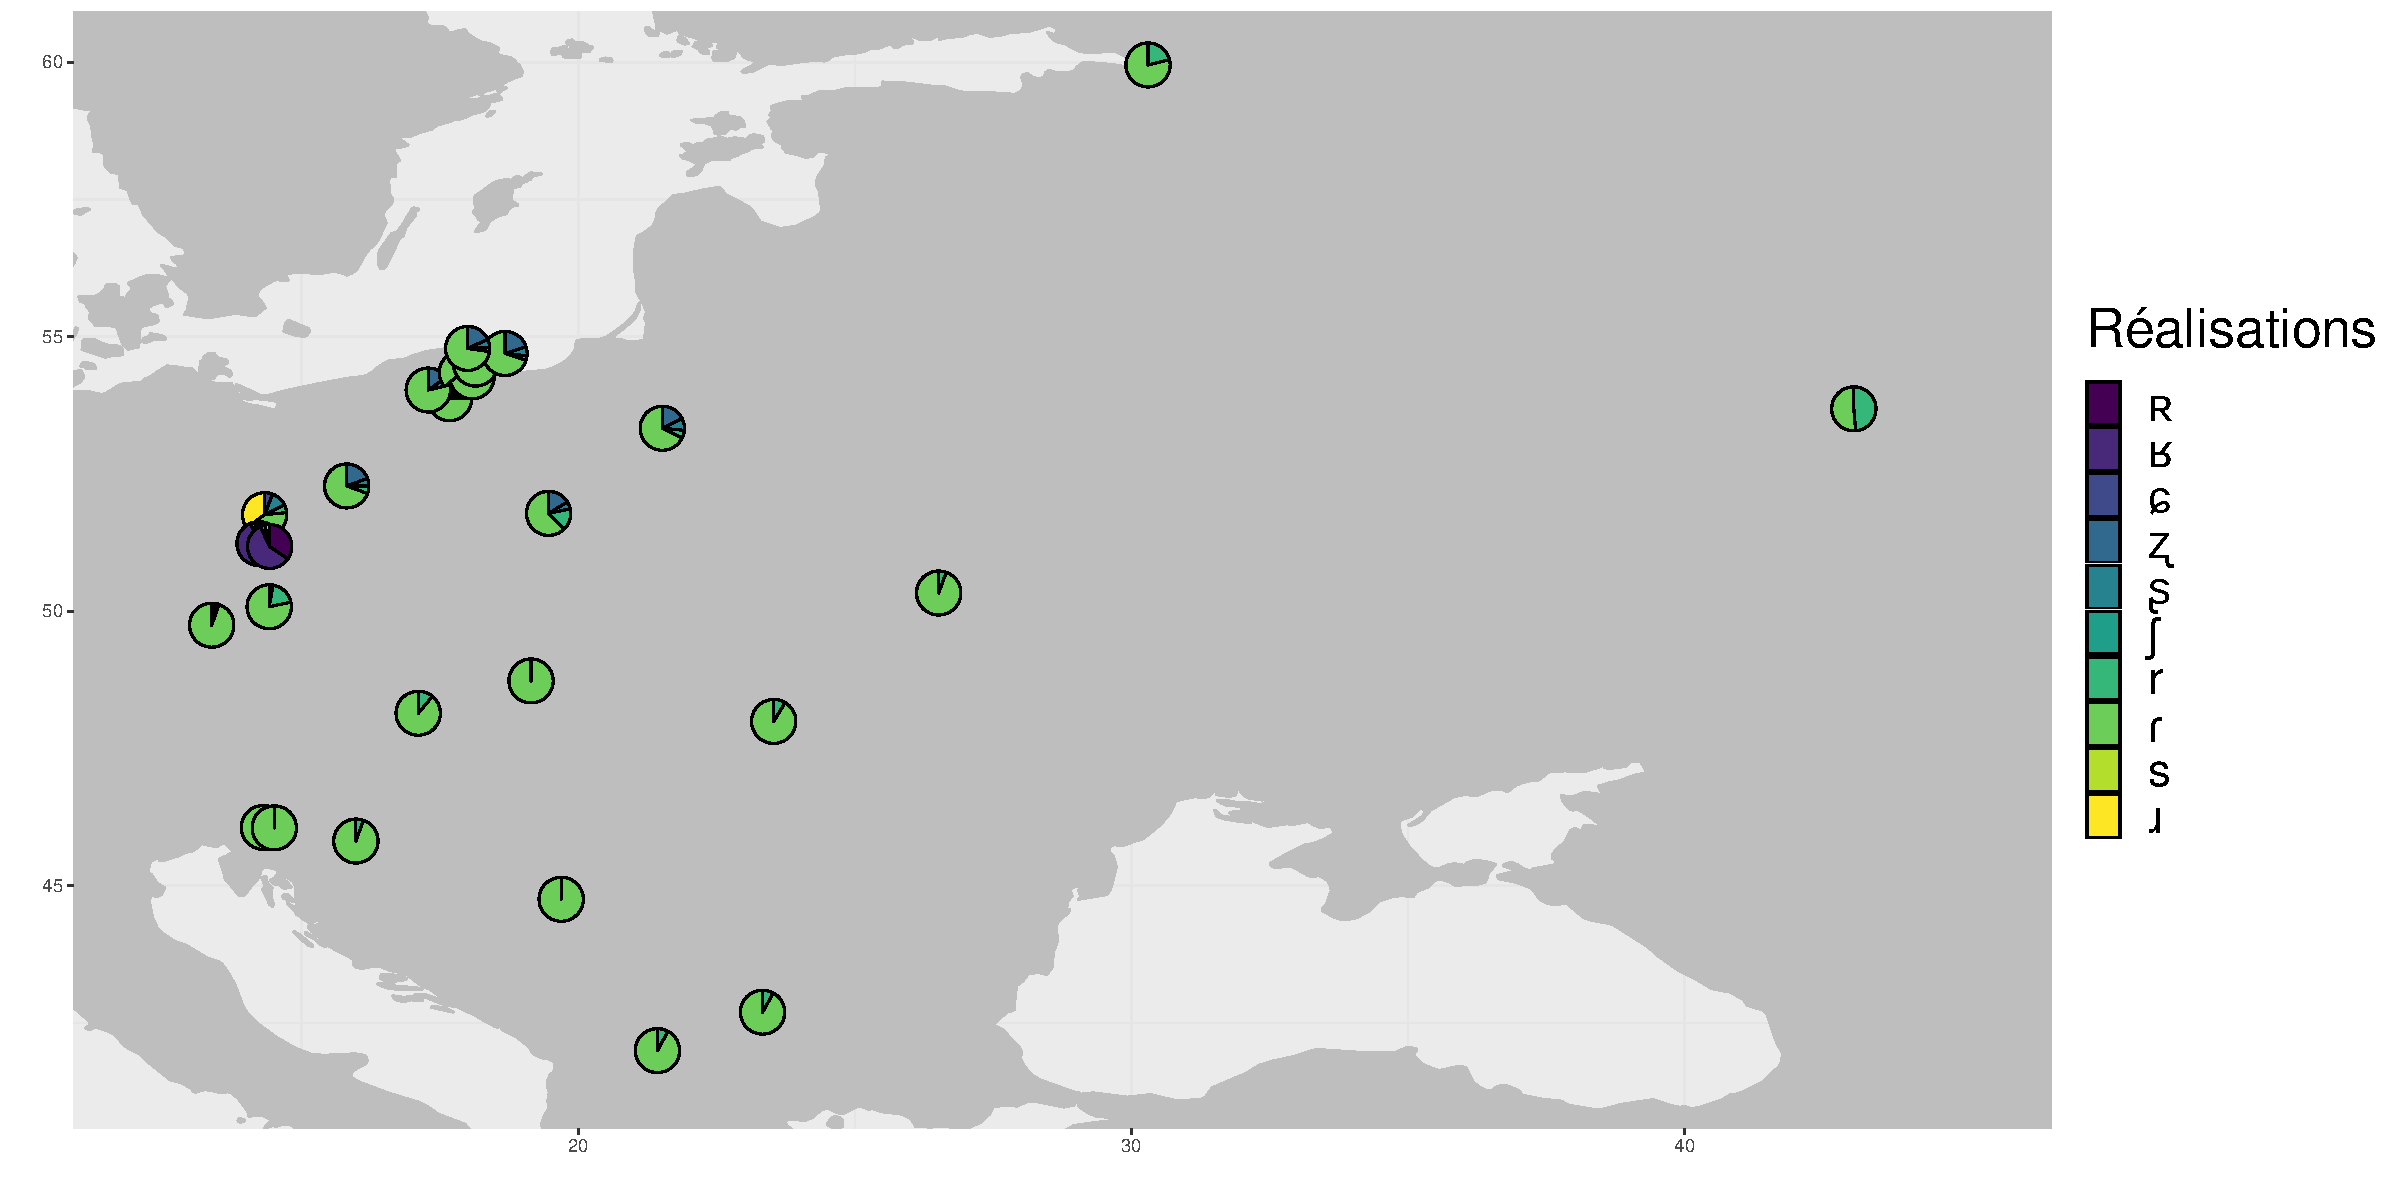
\includegraphics[width=1\linewidth]{substance/images/productionsalvic_1_viridis}
	\caption{Distribution des différentes réalisations dans les variétés slaves étudiées}
	\label{fig:productionsalvic1viridis}
\end{figure}

\begin{figure}
	\centering
	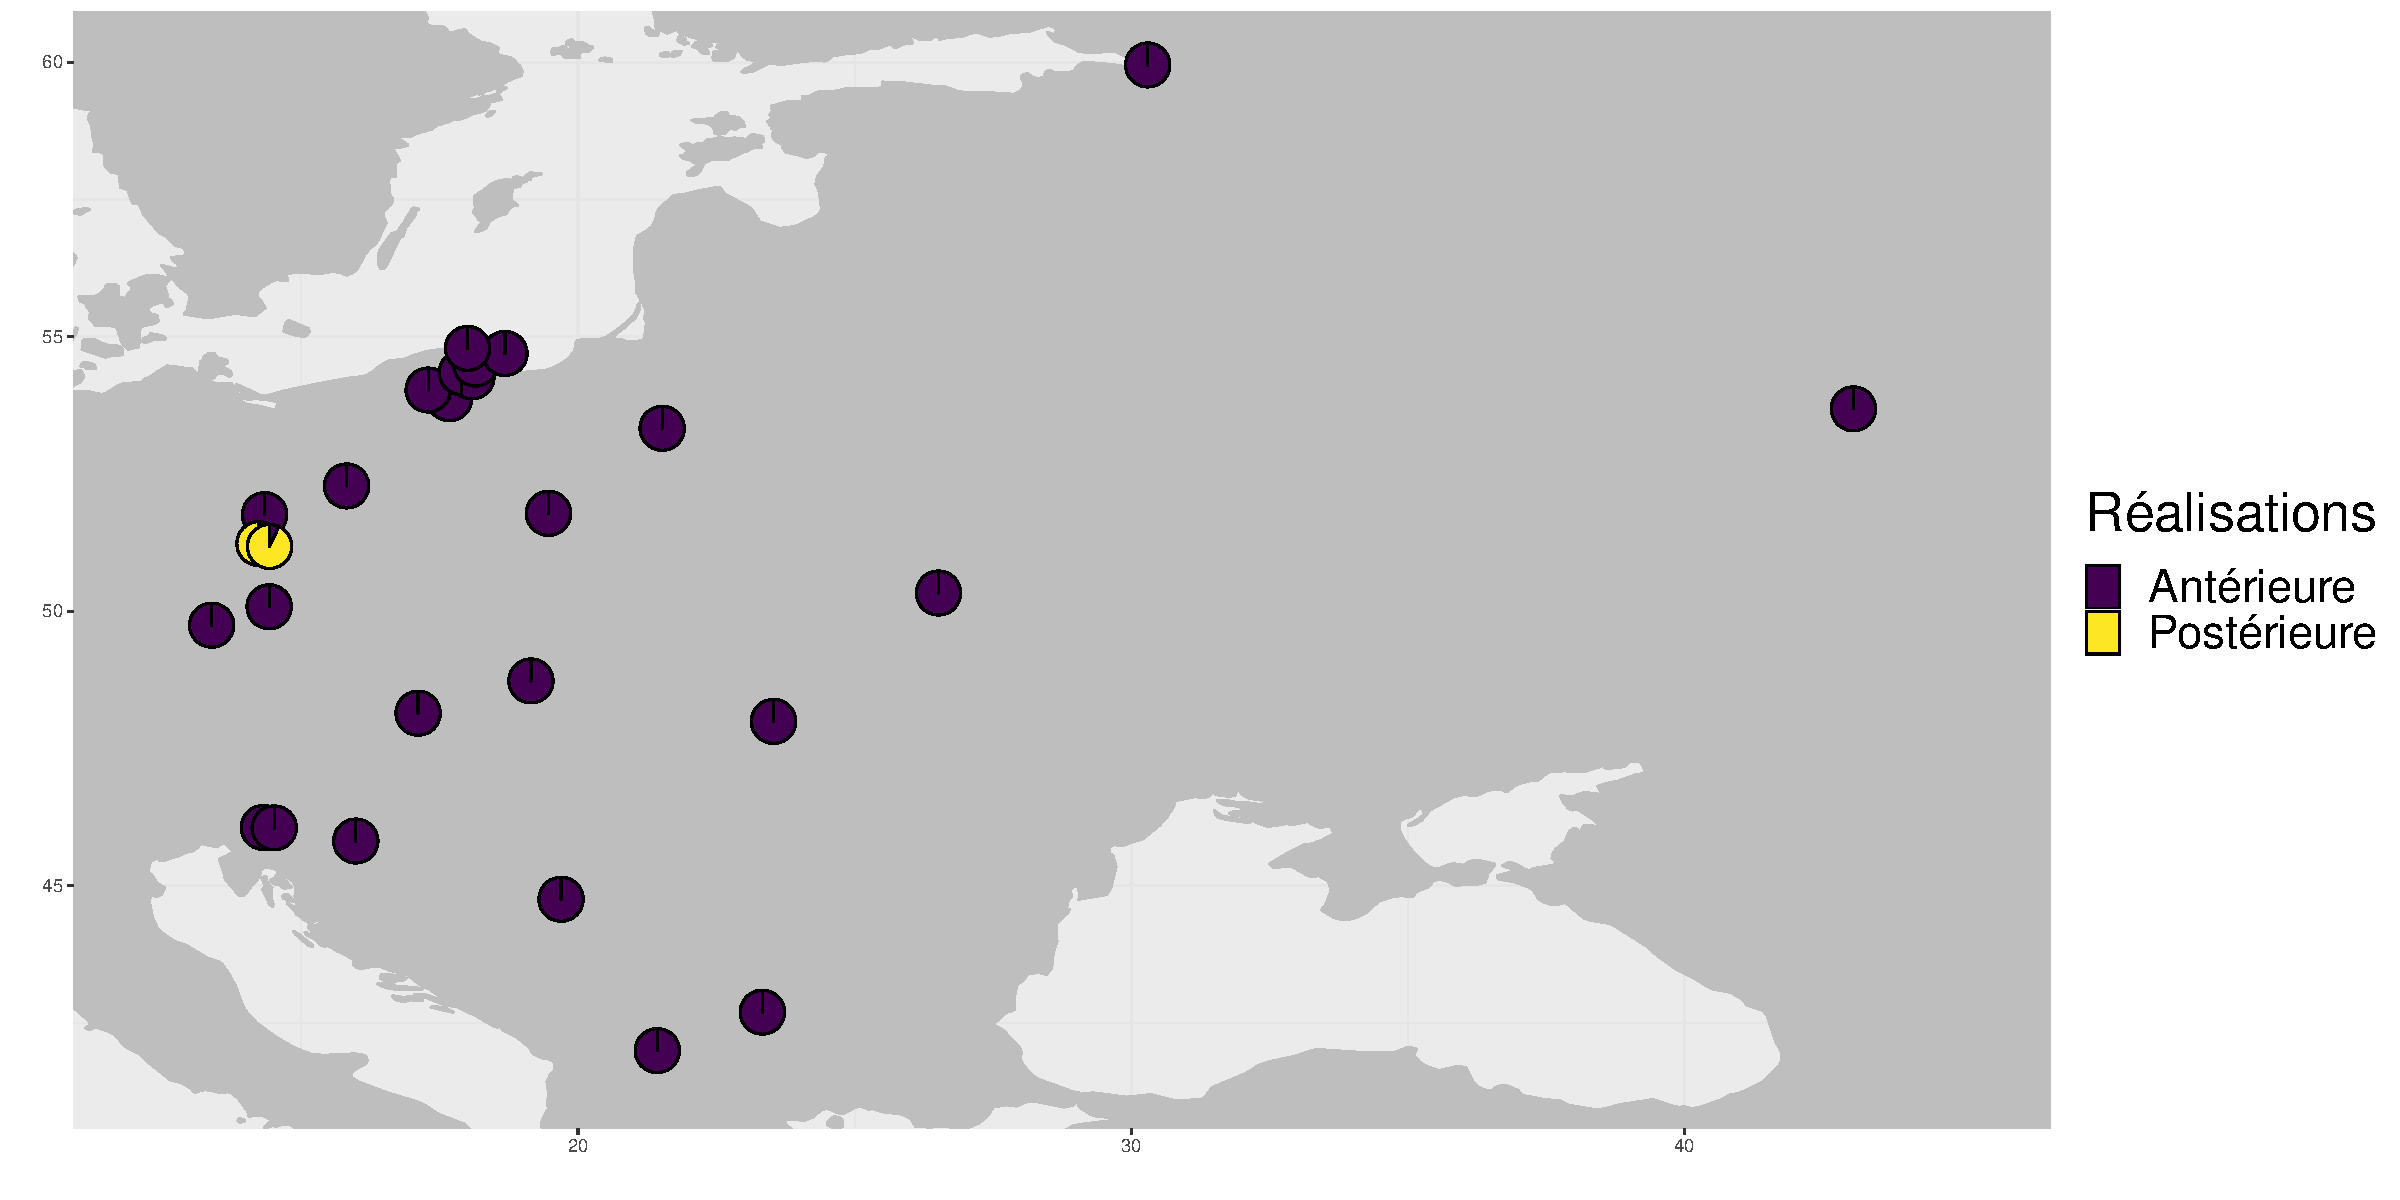
\includegraphics[width=1\linewidth]{substance/images/productionslavic_2_viridis}
	\caption[Distribution des différentes réalisations dans les variétés slaves pour les productions antérieures et postérieures]{Distribution des différentes réalisations dans les variétés slaves étudiées en ne s'intéressant qu'à la dichotomie entre les productions antérieures et postérieures.}
	\label{fig:productionslavic2viridis}
\end{figure}

Les réalisations de la rhotique sont également variées dans les langues slaves (Figure \ref{fig:productionsalvic1viridis}). À l'exception des variétés langagières du haut sorabe parlées en Allemagne, la rhotique est antérieure (Figure \ref{fig:productionslavic2viridis}). Le bas sorabe a conservé une articulation antérieure \parencite{howsonRhoticsPalatalizationAcoustic2018}. \textcite{howsonUpperSorbian2017} oppose deux rhotiques en haut sorabe le /ʀ/ (le hard trill) et le /ʀʲ/ (le soft trill). Les deux phonèmes ont comme allophones [ʀ] et [ʀʲ] mais aussi leurs contreparties approximantes [ʁ] et [ʁʲ]. En plus, le /ʀ/ peut être produit comme une fricative uvulaire sourde [χ]. \textcite{howsonUpperSorbian2017} cite Jocz (2013) (qui, pour rappel, a transcrit les données du slave) en mentionnant que les phonèmes ont tendance à être prononcés comme des trills lorsque la prononciation est soignée, mais qu'il est aussi possible de se retrouver avec une élision de la rhotique palatalisée.  \textcite[440]{schaarschmidtRuleConvergenceLanguage1997} indique que le sorabe n'a plus eu de contact avec une autre langue slave depuis plus de 300 ans mais était en contact avec l'allemand. Il est plausible que la postériorité de l'articulation de la rhotique soit une conséquence de ce contact.\\


\begin{figure}
	\centering
	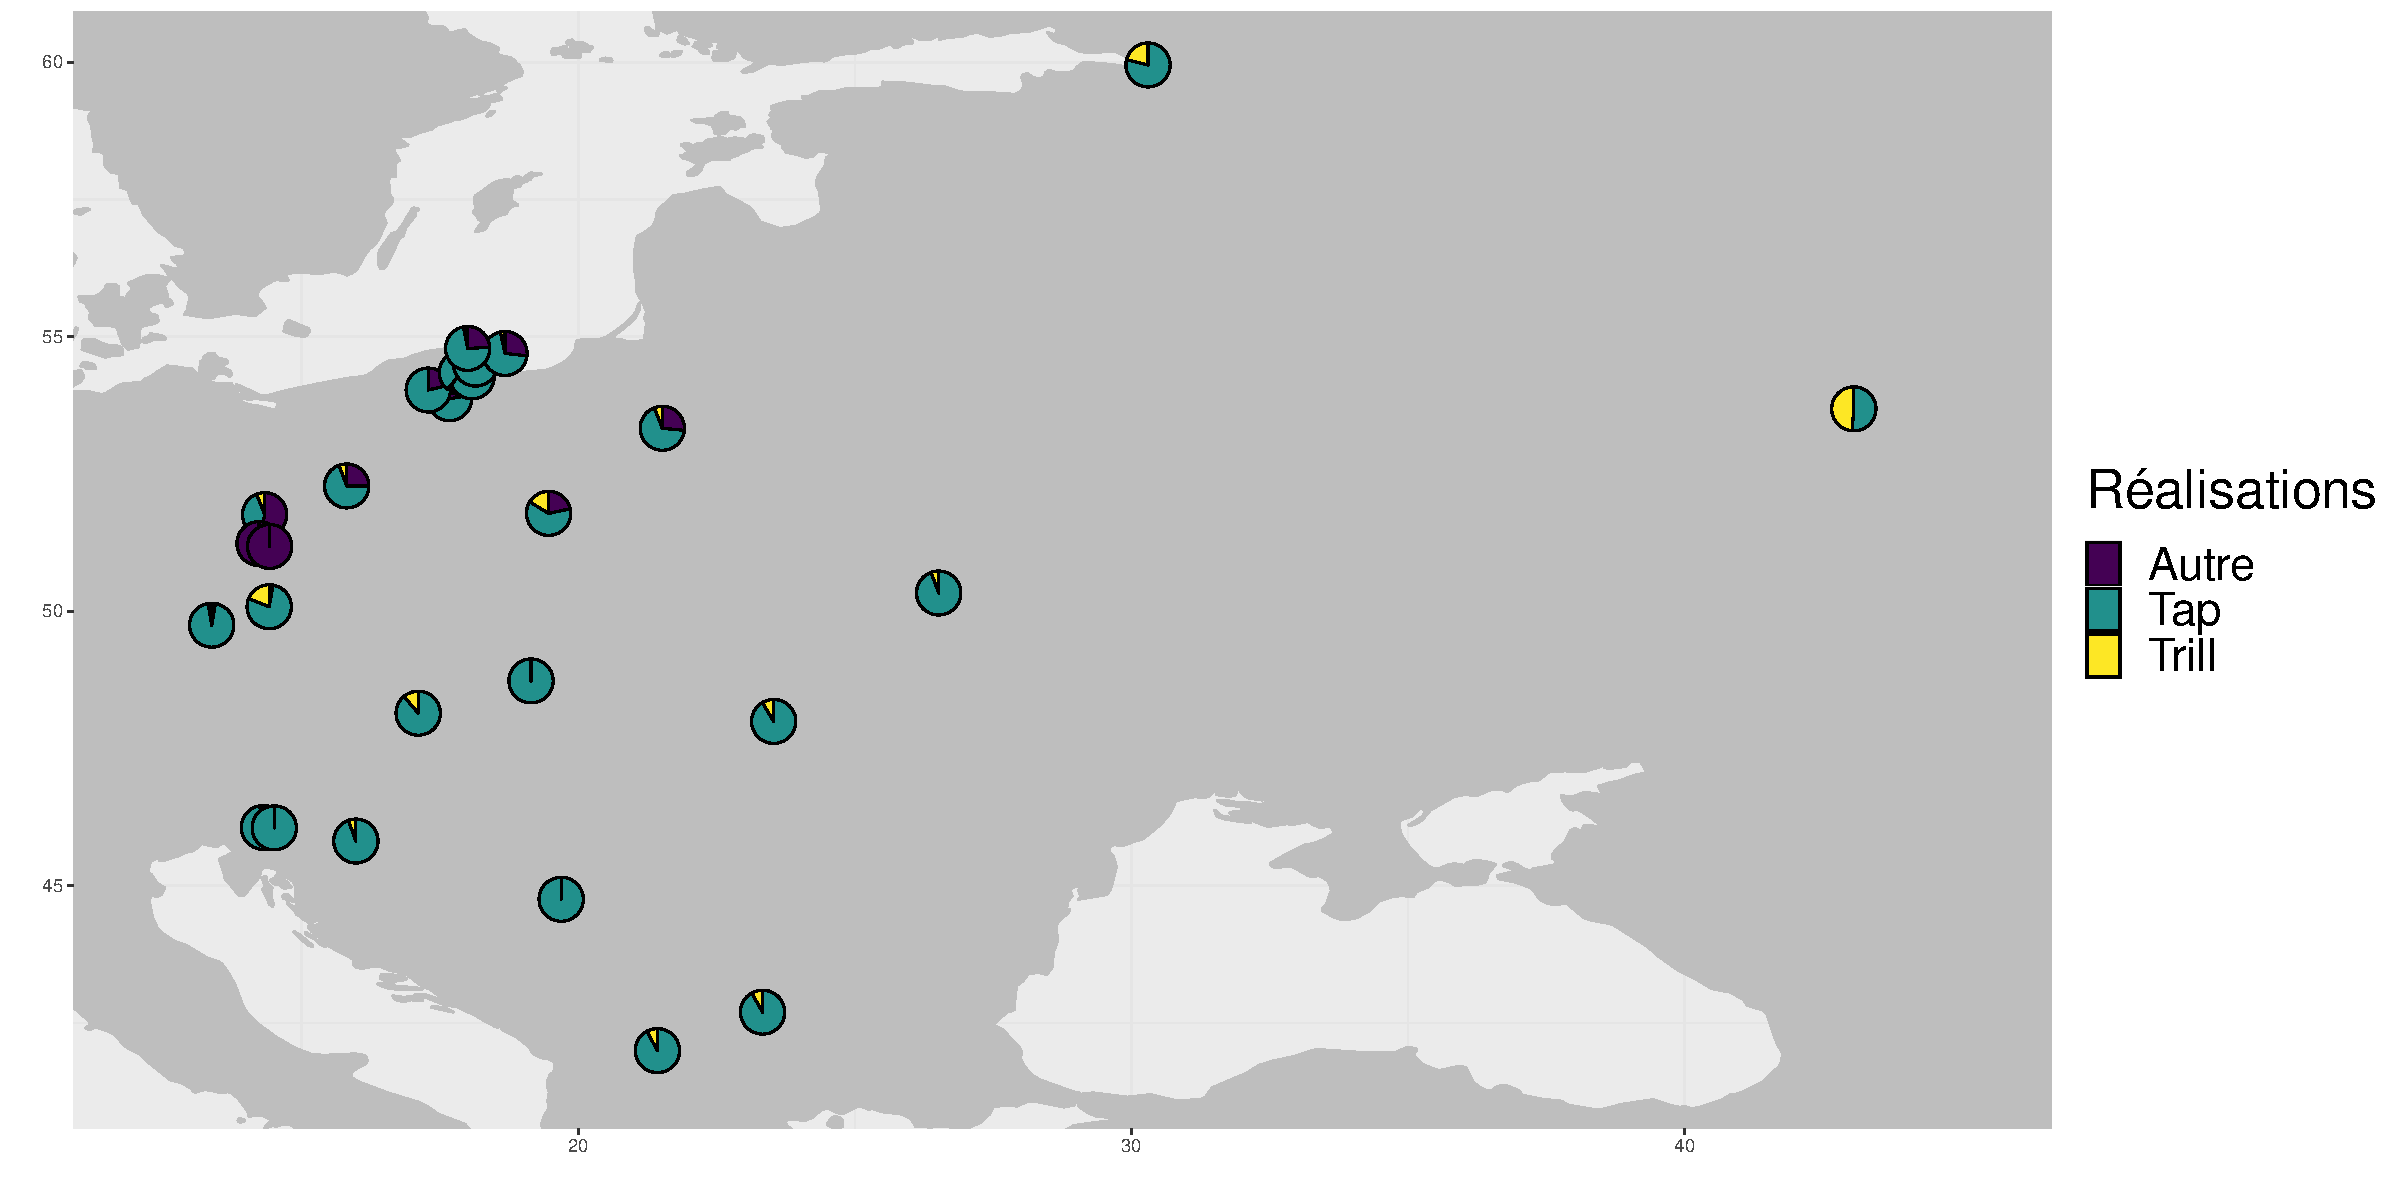
\includegraphics[width=1\linewidth]{substance/images/productionslavic_3_viridis}
	\caption[Distribution des différentes réalisations dans les variétés slaves pour le trill et tap]{Distribution des différentes réalisations dans les variétés slaves étudiées en ne s'intéressant qu'à la dichotomie entre trill et tap (et les autres segments).}
	\label{fig:productionslavic3viridis}
\end{figure}

\begin{figure}
	\centering
	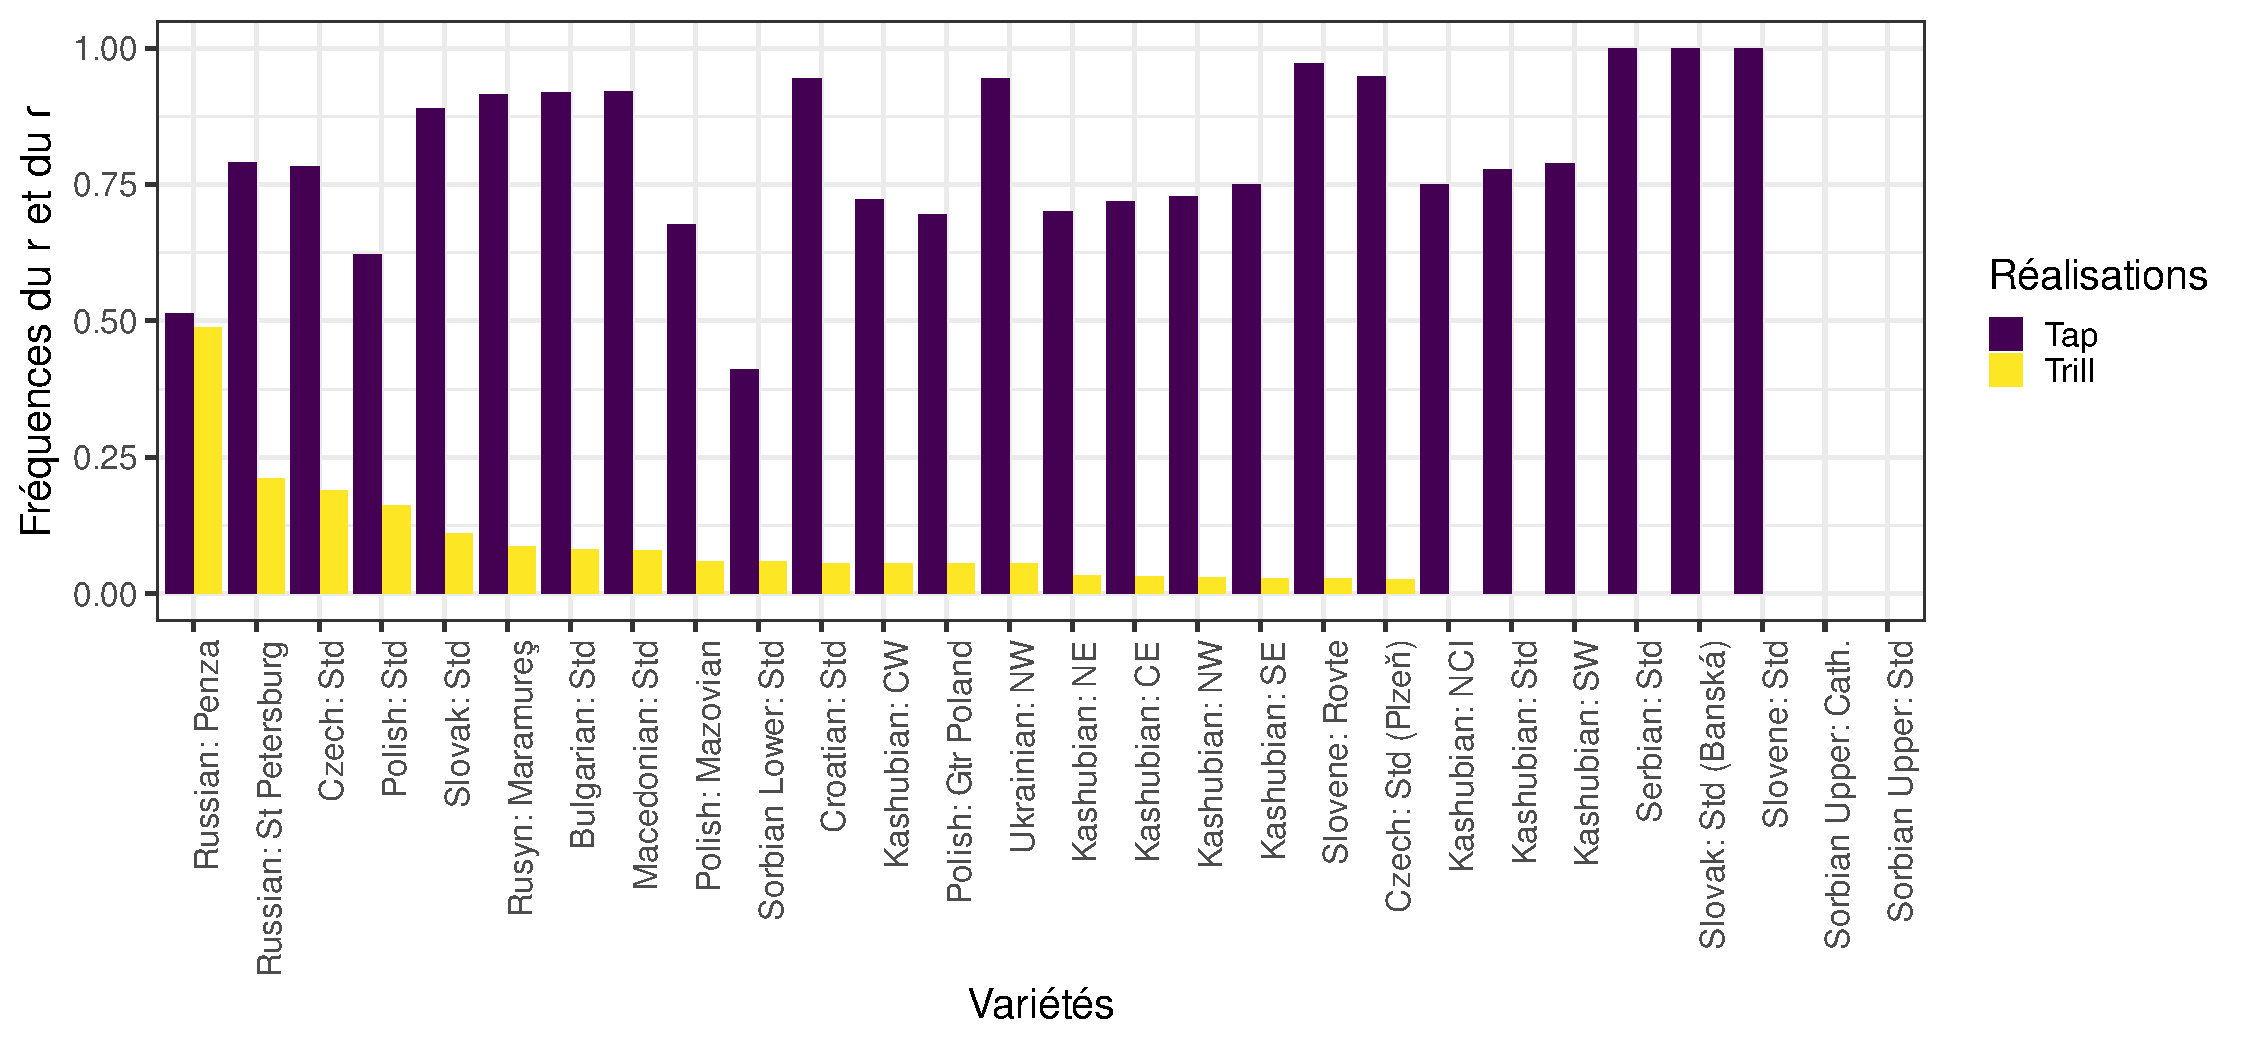
\includegraphics[width=1\linewidth]{substance/images/freq_trill_slavic2}
	\caption[Fréquences du trill et du tap dans les variétés slaves]{Fréquences du trill et du tap dans les variétés slaves. Seules les variétés où au moins 1/3 des transcriptions ont été faites sont incluses.}
	\label{fig:freqtrillslavic}
\end{figure}

Lorsqu'on s'intéresse spécifiquement aux variétés qui ont des réalisations antérieures pour la rhotique, on remarque que de manière similaire aux variétés romanes, la rhotique majoritaire est le tap (\autoref{fig:productionslavic3viridis}). Le trill peut être présent dans certains cas. C'est dans la variété de russe parlée à \href{https://soundcomparisons.com/#/en/Slavic/language/BSv_SvE_Rus_C_Pen_Vadinsk_Dl}{Panza} qu'on retrouve le plus de trills.
En supprimant les variétés sans aucun trill, la moyenne de la fréquence du trill est à 0,09, sa médiane à 0,06 et son écart inter-quartile de 0,06 (Figure \ref{fig:freqtrillslavic}).
Pour le tap, dans ces mêmes variétés où on a des trills, sa fréquence moyenne est à 0,78, sa fréquence médiane est à 0,77 et son écart inter-quartile est de 0,22.\\

\subsection{Cas du latin classique}

Le statut de la rhotique en latin ainsi que dans les reconstructions n'est pas un sujet nouveau. 
De nombreux auteurs contemporains au latin ont laissé des indications sur la production de la rhotique qui suggèrent un trill comme réalisation systématique de la rhotique.
Néanmoins, de manière similaire à l'anglais d'Écosse, il n'est pas impossible que les locuteurs et locutrices de l'époque n'aient pas eu de vision globale des différents variants qu'ils et elles utilisaient.
Il nous est apparu que le latin classique faisait figure d'exception. Lorsqu'on regarde la Figure \ref{fig:productionromane3viridis}, le latin apparaît dans tous les cas avec un trill, à l'exception d'une occurrence où il s'agit d'un tap que nous considérons comme étant une erreur de transcription. \\

\textcite{juretPhonetiqueLatine1938} dans son ouvrage \textit{La phonétique latine} mentionne qu'on ne trouvait qu'un type de \textit{r} en latin, un \textit{r} produit comme celui de l'italien et des langues romanes de manière générale. Juret décrit le \textit{r} comme une vibrante avec des « vibrations de la pointe de la langue avancée vers les alvéoles » (p. 14). Il y mentionne aussi que le \textit{r} a pu être impliqué dans un phénomène de gémination à valeur expressive, et il semblerait que la langue a conservé cette variante dans certains de ses mots au dépit de la variante simple (p. 89). Bien que le terme trill ne soit pas utilisé, on peut inférer qu'il ait pu exister, en latin, deux phones contrastant principalement par la longueur, probablement un tap et un trill. \\

\textcite{pultrovaPhoneticNatureLatin2013} s'interroge sur la littérature latiniste affirmant que le \textit{r} latin était un tap en observant les rhotiques produites en synchronie dans les langues romanes. \citeauthor{pultrovaPhoneticNatureLatin2013} démontre sur la base de la lecture critique d'auteurs latinistes et d'analyses linguistiques que le \textit{r} latin était alvéolaire plutôt qu'uvulaire. Il s'agissait d'un tap/flap plutôt que d'un trill. Cependant, l'autrice échoue à mettre en évidence la double nature de la rhotique. Bien que dans la majorité des cas la rhotique ait pu être produite comme un tap, il n'en restait pas moins possible de la produire comme un trill.\\

\textcite{canepariPronunciaNeutraInternazionale2008} (p. 5) nous semble être le premier à donner [r] et [ɾ] comme symboles de l'API possibles pour la transcription du /r/. Dans ses transcriptions, il réserve le [r] aux syllabes accentuées et le [ɾ] aux syllabes non accentuées (page 7). Dans le cas de la gémination, sa règle s'applique aussi. /ɪrriːˈtaːt/ donne [ˌɪɾɾiˈtaˑt] et /ɪrˈriːtɐt/ donne [ɪɾˈriːtɐt]. Canepari transcrit la Bise et le Soleil en latin. Dans sa transcription du latin classique, on retrouve 33 occurrences de la rhotique dont 4 trills (12\%) et 29 taps (88\%). La fréquence du trill est beaucoup plus ressemblante à ce que nous avons trouvé avec les variétés romanes enregistrées de Sound Comparisons, où la moyenne était de 18\% et la médiane de 13\%.\\

Dans le tableau \ref{tab:productionclassicallatin}, nous donnons des exemples de transcriptions reconstruites par Sound Comparisons. Le [ɾ] n'apparaît que dans deux cognats, et le [r] est systématiquement utilisé indépendamment de la position de la rhotique dans le mot et la syllabe, et du poids syllabique. Si l'on s'en tient aux propos de Canepari, il y a de nombreuses transcriptions où le \textit{r} est donné divergent de ce qui aurait pu être attendu (n = 16 contre n = 21 non divergentes). 
Nous estimons que concernant la rhotique, ces transcriptions de Sound Comparisons relèvent plus de transcriptions larges qu'étroites contrairement aux attentes que nous aurions pu avoir.\\

\begin{table}
	\centering
	\resizebox{\linewidth}{!}{
	\csvautobooktabular{substance/tables/production_classical_latin.csv}}
	\caption[Transcriptions de certains cognats utilisés dans Sound Comparison avec une correction basée selon la règle de Canepari (2008)]{Transcriptions de certains cognats utilisés dans Sound Comparisons avec une correction basée selon la règle de \textcite{canepariPronunciaNeutraInternazionale2008}.}
	\label{tab:productionclassicallatin}
\end{table}

En conclusion de cette sous-section sur le latin classique, nous pensons qu'il n'est pas invraisemblable que les différents allophones en latin aient eu une distribution similaire à celle qu'on retrouve en italien ou en espagnol contemporain.
%Et bien que cela se base sur le fait que trill s'y retrouve dans les syllabes toniques et le tap dans les syllabes atoniques, nous n'avons pas développé la possibilité de l'inverse sur la base du gascon \parencite{mooneyBearnaisGascon2014} où c'était le tap qui se retrouvait en syllabe tonique et le trill en syllabe atonique.


\section{Etude de cas 3 : le cas des langues germaniques}

Nous nous sommes aussi intéressé à un autre ensemble de langues pour lesquelles la transcription était moins étroite que pour les variétés romanes et slaves. Il s'agit des langues germaniques.

\subsection{Description des langues germaniques}

Les variétés de langues germaniques couvertes par Sound Comparisons sont vastes. On y retrouve les variétés parlées en Scandinavie \parencites{engstrandSwedish1990,gronnumDanish1998,basbollPhonologyDanish2005,kristjanarnasonPhonologyIcelandicFaroese2011}, dans les îles britanniques et aux États-Unis d'Amérique (cf. les dialectes de l'anglais ont une {\href{https://soundcomparisons.com/#/en/Englishes/map/red/Lgs_Sln}{étude dans Sound Comparisons}} qui leur est entièrement dédiée avec plus d'enregistrements et de transcriptions) \parencite{decampAmericanEnglishEastern1973,nallyNotesWestmeathDialect1971,hillenbrandAmericanEnglishSouthern2003,wattTynesideEnglish2003,roachBritishEnglishReceived2004,watsonLiverpoolEnglish2007}. On retrouve aussi des variétés du frisian \parencite{petersSaterlandFrisian2019}, du néerlandais \parencite{meesPhoneticDescriptionConsonant1982,gussenhovenDutch1992,heijmansDutchDialectWeert1998,verhoevenBelgianStandardDutch2005}, du flamand \parencite{petersFlemishBrabantDialectOrsmaalGussenhoven2010}, de l'afrikaans \parencite{wissingAfrikaans2020}, du bavarois \parencite{galataAcousticAnalysisTyrolean2016} ou encore de l'allemand \parencite{kohlerGerman1990,khanUpperSaxonChemnitz2013}.\\

Les rhotiques varient en fonction de l'aire géographique. Pour les langues germaniques de Scandinavie, on retrouve le trill voisé et non voisé en islandais alors qu'il est absent en féroïen où on retrouve des productions approximantes. De même, en suédois, il est possible d'entendre un trill dans certains contextes emphatiques. Historiquement, toutes ces variétés ont pu avoir un trill comme c'est le cas pour le danois \parencite[218]{basbollPhonologyDanish2005}, alors que de nos jours on ne retrouve plus de trill ou de tap/flap comme allophone d'une rhotique (p. 126).
Les approximantes sont présentes dans les variétés de l'anglais des îles britanniques, même si on peut retrouver d'autres variants dans les contextes emphatiques comme des fricatives, des tap/flaps, ou même des trills.
Dans les variétés du néerlandais, ce sont principalement des trills alvéolaires, qui sont en variation libre avec des trills uvulaires. La thèse en sociophonétique de \textcite{sebregtsSociophoneticsPhonologyDutch2014} s'intéresse à la variation des rhotiques en néerlandais. Son corpus est composé de productions issues de dix accents urbains du néerlandais et lui permet de mettre en évidence vingt variants du \textit{r} (dont des voyelles slaves et des élisions avec ou sans effet sur la consonne suivante) bien que \citeauthor{sebregtsSociophoneticsPhonologyDutch2014} note justement :

\begin{displayquote}
	Decisions as to how many variants to code for were influenced by the perceived need to make distinctions and constrained by the degree of difficulty in distinguishing variants. \parencite[284]{sebregtsSociophoneticsPhonologyDutch2014}
\end{displayquote}

Ses résultats globaux montrent que parmi les variants majeurs on retrouve \textit{ɾ}, \textit{ʁ̞}, \textit{ɻ}~~ et \textit{ʀ}. Le trill [r] n'est pas présent parmi les variants majeurs. La plupart des accents urbains mettent en évidence la variation entre les productions alvéolaires et uvulaires, bien que dans certains accents les productions soient majoritairement soit alvéolaires, soit uvulaires.\\

Les variétés de l'allemand sont aussi confrontées à beaucoup de variation avec des productions généralement uvulaires avec plus ou moins de friction et avec de la variation contextuelle. \\

Contrairement aux variétés slaves et romanes, beaucoup de personnes ont été impliquées dans les transcriptions des langues germaniques. Il nous est apparu que ces personnes n'ont pas comme spécialité la dialectologie. On y retrouve deux transcripteurs principaux \href{http://www.ludgerpaschen.de/}{Ludger Paschen} et \href{https://www.researchgate.net/profile/Jan-Michalsky}{Jan Michalsky}, et des collaborateurs et collaboratrices.\\
Les transcriptions des variétés d'Allemagne centrale et de l'est ont été effectuées par \href{http://www.ludgerpaschen.de/}{Ludger Paschen}. Sa \href{https://www.ludgerpaschen.de/papers/Paschen2018_PhD.pdf}{thèse} \parencite{paschenInteractionReduplicationSegmental2018} porte sur l'interaction entre la réduplication et les mutations segmentales. Dans Sound Comparisons, il a aussi transcrit d'autres variétés germaniques.
\href{https://www.researchgate.net/profile/Jan-Michalsky}{Jan Michalsky} a aussi contribué à la transcription des variétés continentales germaniques de l'ouest. Sa \href{https://www.degruyter.com/document/doi/10.1515/9783110538564/html}{thèse} \parencite{michalskyFrageintonationImDeutschen2017} porte sur les intonations dans les questions en allemand.\\

\href{https://gns.wisc.edu/person/matthew-boutilier/}{Matthew Boutilier} a travaillé aux transcriptions reconstruites des langues historiques germaniques et prépare son doctorat en linguistique historique germanique.
\href{http://www.lel.ed.ac.uk/~wmaguire/}{Warren Maguire} a contribué avec les transcriptions des diffférentes variétés de l'anglais.
Darja Dërmaku-Appelganz, \href{https://www.coli.uni-saarland.de/~evaly/}{Eva Lasarcyk}, \href{https://florianmatter.gitlab.io/}{Florian Matter}, \href{https://www.davidcrystal.com/GBR/David-Crystal}{David Crystal}, Han Nijdam et Philippe Simon ont eux aussi contribué aux transcriptions.\\

\subsection{Résultats de la caractérisation de la rhotique dans les langues germaniques}

\begin{figure}
	\centering
	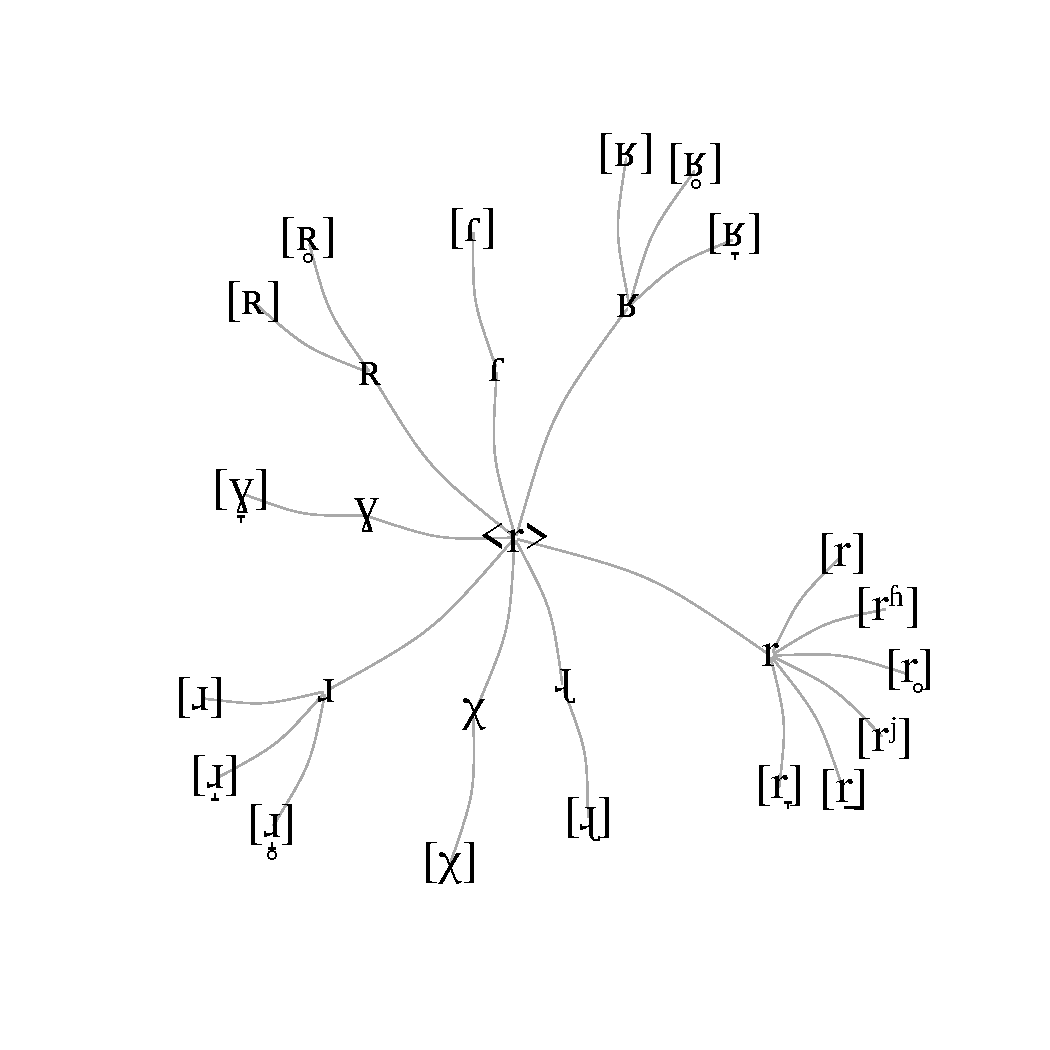
\includegraphics[width=0.7\linewidth]{substance/images/germanic_rhotics}
	\caption[Graphe des différentes réalisations de la rhotique dans les variétés germaniques]{Graphe des différentes réalisations de la rhotique dans les variétés germaniques à partir des données de Sound Comparisons. Nous représentons uniquement les réalisations de la rhotique quand elle est en position initiale ou en deuxième position d'attaque branchante. Le graphe est obtenu avec le package \texttt{igraph} \parencite{csardiIgraphSoftwarePackage2006}.}
	\label{fig:germanicrhotics}
\end{figure}

La figure \ref{fig:germanicrhotics} obtenue à partir des données de Sound Comparisons nous permet de  mettre en évidence que huit caractères forment le niveau d'analyse intermédiaire. Au total, il y a 18 réalisations possibles pour les différents cognats pris en compte.
Quatre lieux d'articulations sont possibles avec les rhotiques alvéolaire, rétroflexe, vélaire et uvulaire, pour quatre manières d'articulation avec les trills, les taps, les fricatives et les approximantes.
En moyenne chaque caractère intermédiaire possède environ 2,25 réalisations.\\

\begin{figure}
	\centering
	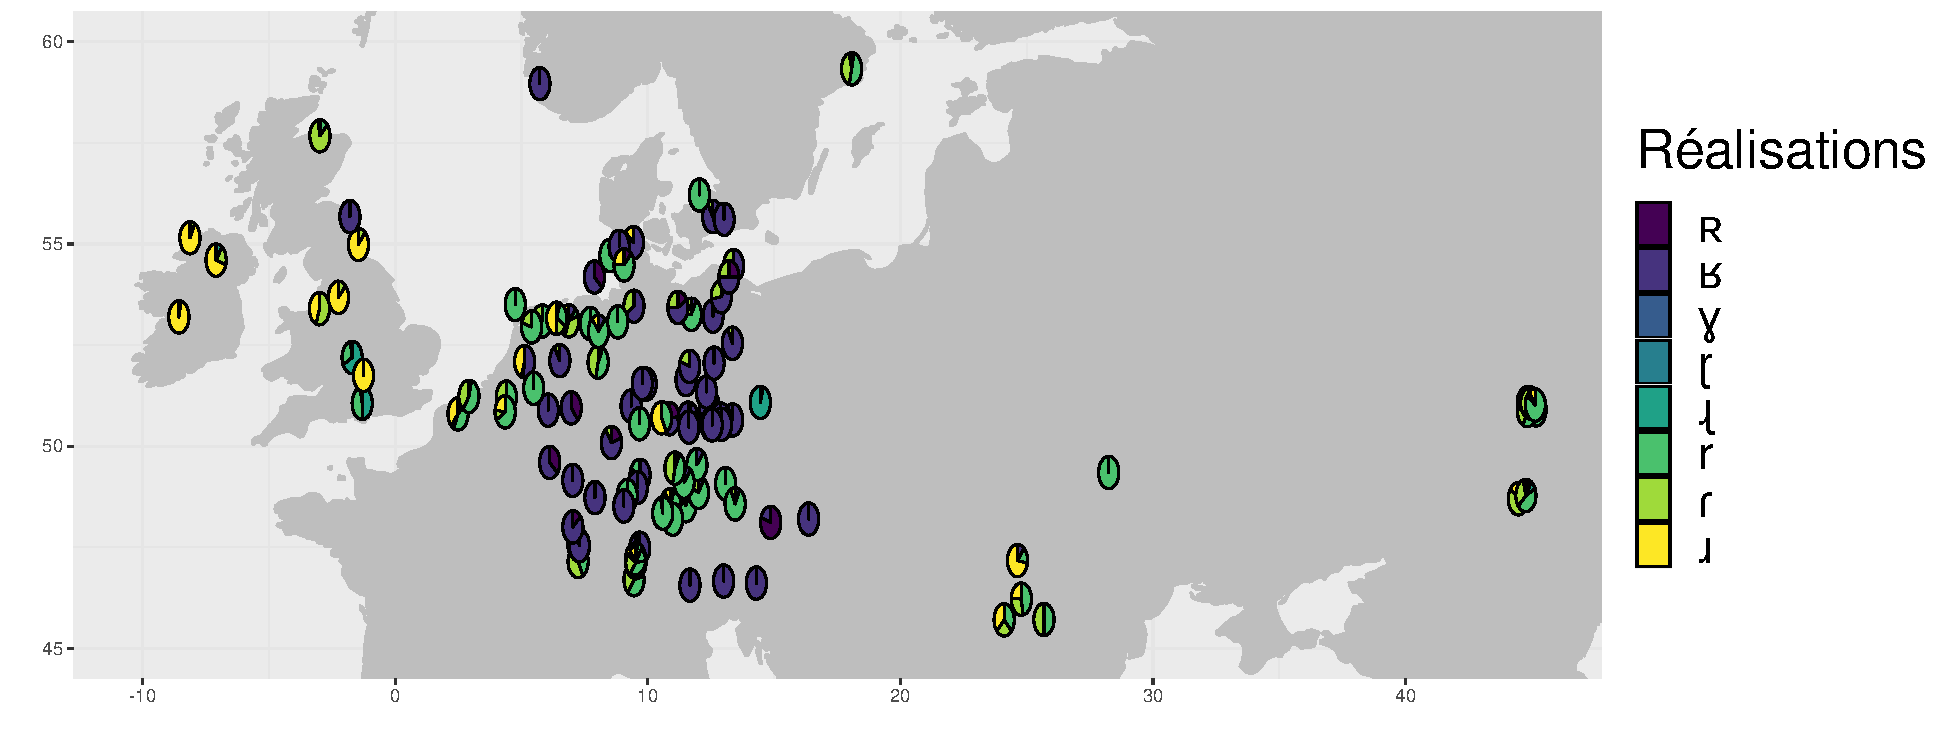
\includegraphics[width=1\linewidth]{substance/images/productiongermanic_1_viridis}
	\caption[Distribution des différentes réalisations dans les variétés germaniques]{Distribution des différentes réalisations dans les variétés germaniques étudiées. La carte montre seulement les variétés parlées en Europe continentale.}
	\label{fig:productiongermanic1viridis}
\end{figure}

\begin{figure}
	\centering
	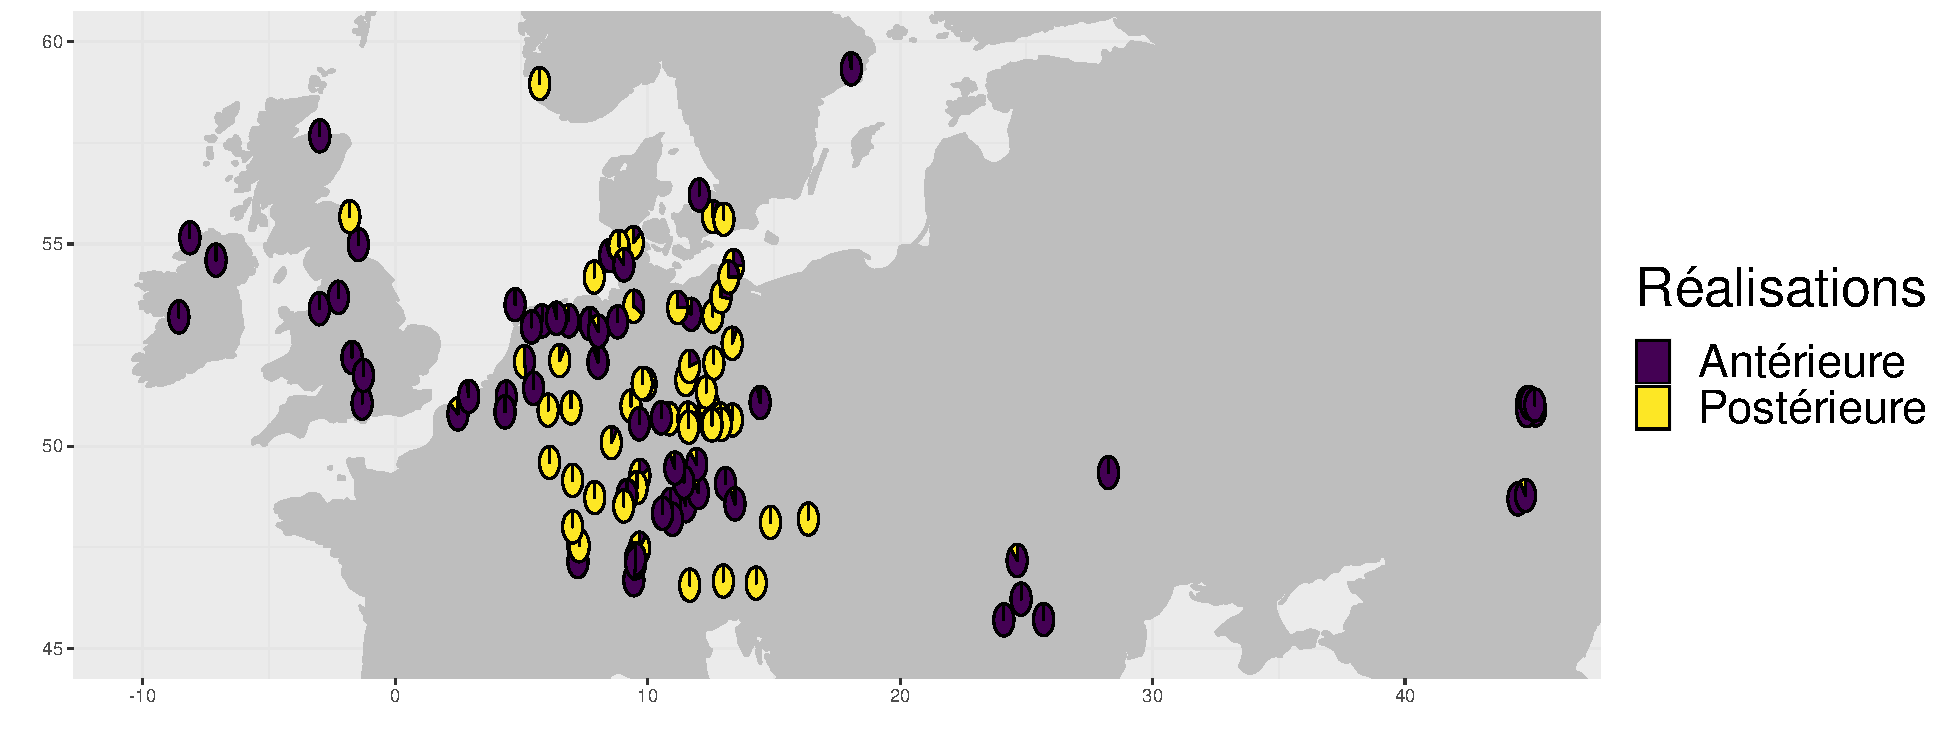
\includegraphics[width=1\linewidth]{substance/images/productiongermanic_2_viridis}
	\caption[Distribution des différentes réalisations dans les variétés germaniques pour les productions antérieures et postérieures]{Distribution des différentes réalisations dans les variétés germaniques étudiées en ne s'intéressant qu'à la dichotomie entre les productions antérieures et celles postérieures (et l'absence de segment).}
	\label{fig:productiongermanic2viridis}
\end{figure}

L'ensemble des variétés germaniques ne produit pas uniquement des consonnes antérieures ou des consonnes postérieures. 
On retrouve en Allemagne une majorité de variétés enregistrées avec des productions postérieures, mais on retrouve, dans le sud du pays, de l'antériorité dans les consonnes. À l'extérieur de l'Allemagne, ce sont les variétés avec un lieu d'articulation antérieur qui sont représentées.\\

\begin{figure}
	\centering
	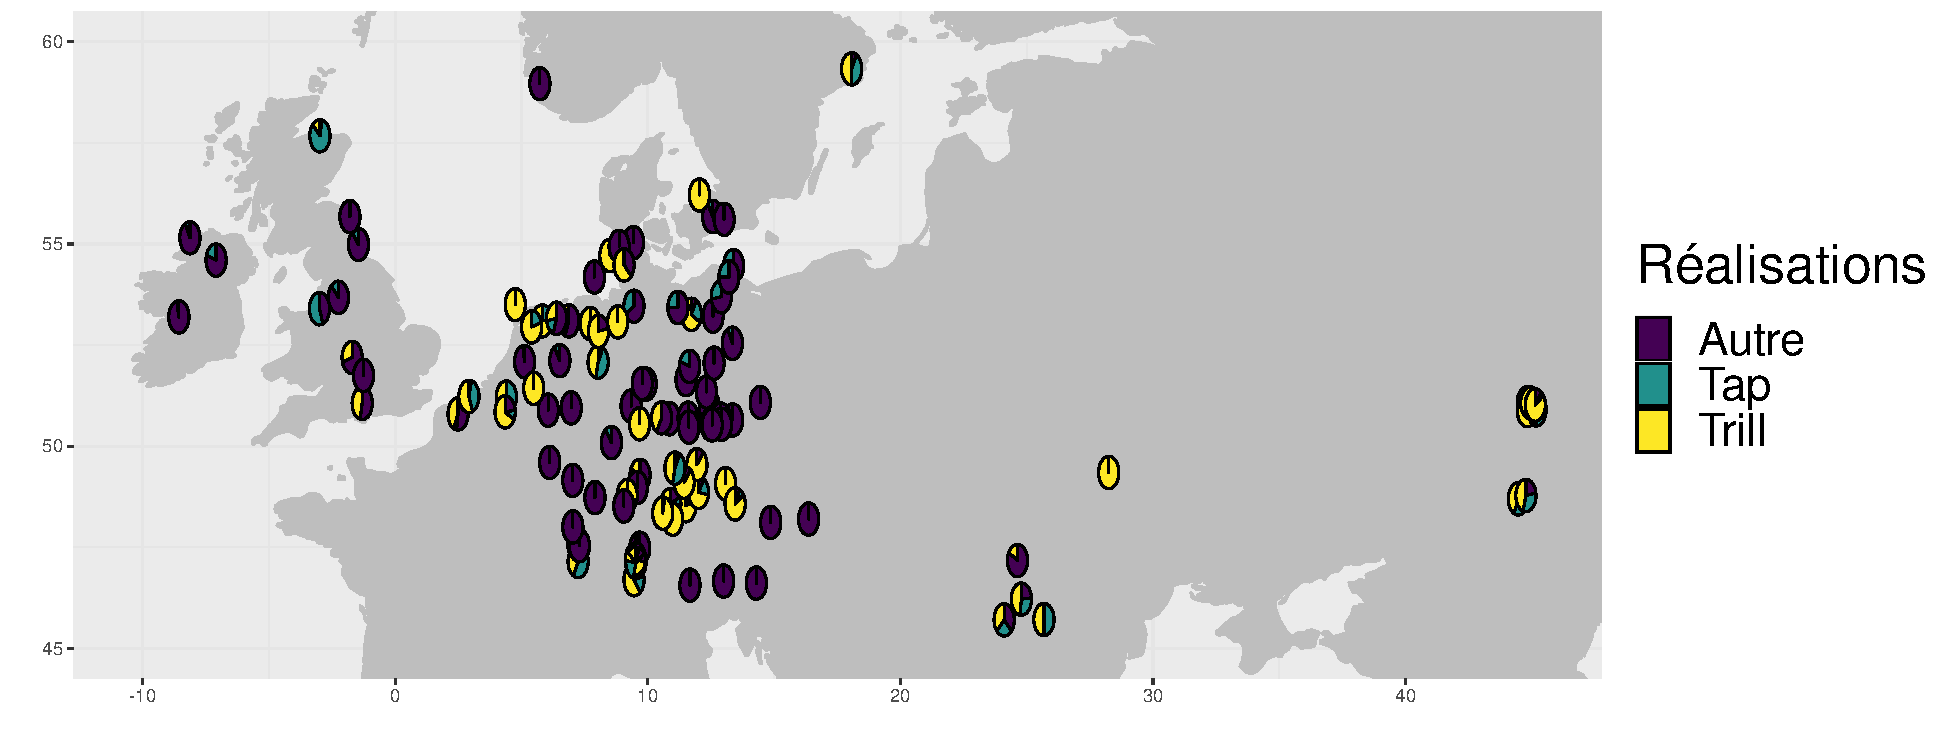
\includegraphics[width=1\linewidth]{substance/images/productiongermanic_3_viridis}
	\caption[Distribution des différentes réalisations dans les variétés germaniques pour le trill et le tap]{Distribution des différentes réalisations dans les variétés germaniques étudiées en ne s'intéressant qu'à la dichotomie entre trill et tap (et les autres segments).}
	\label{fig:productiongermanic3viridis}
\end{figure}

\begin{figure}
	\centering
	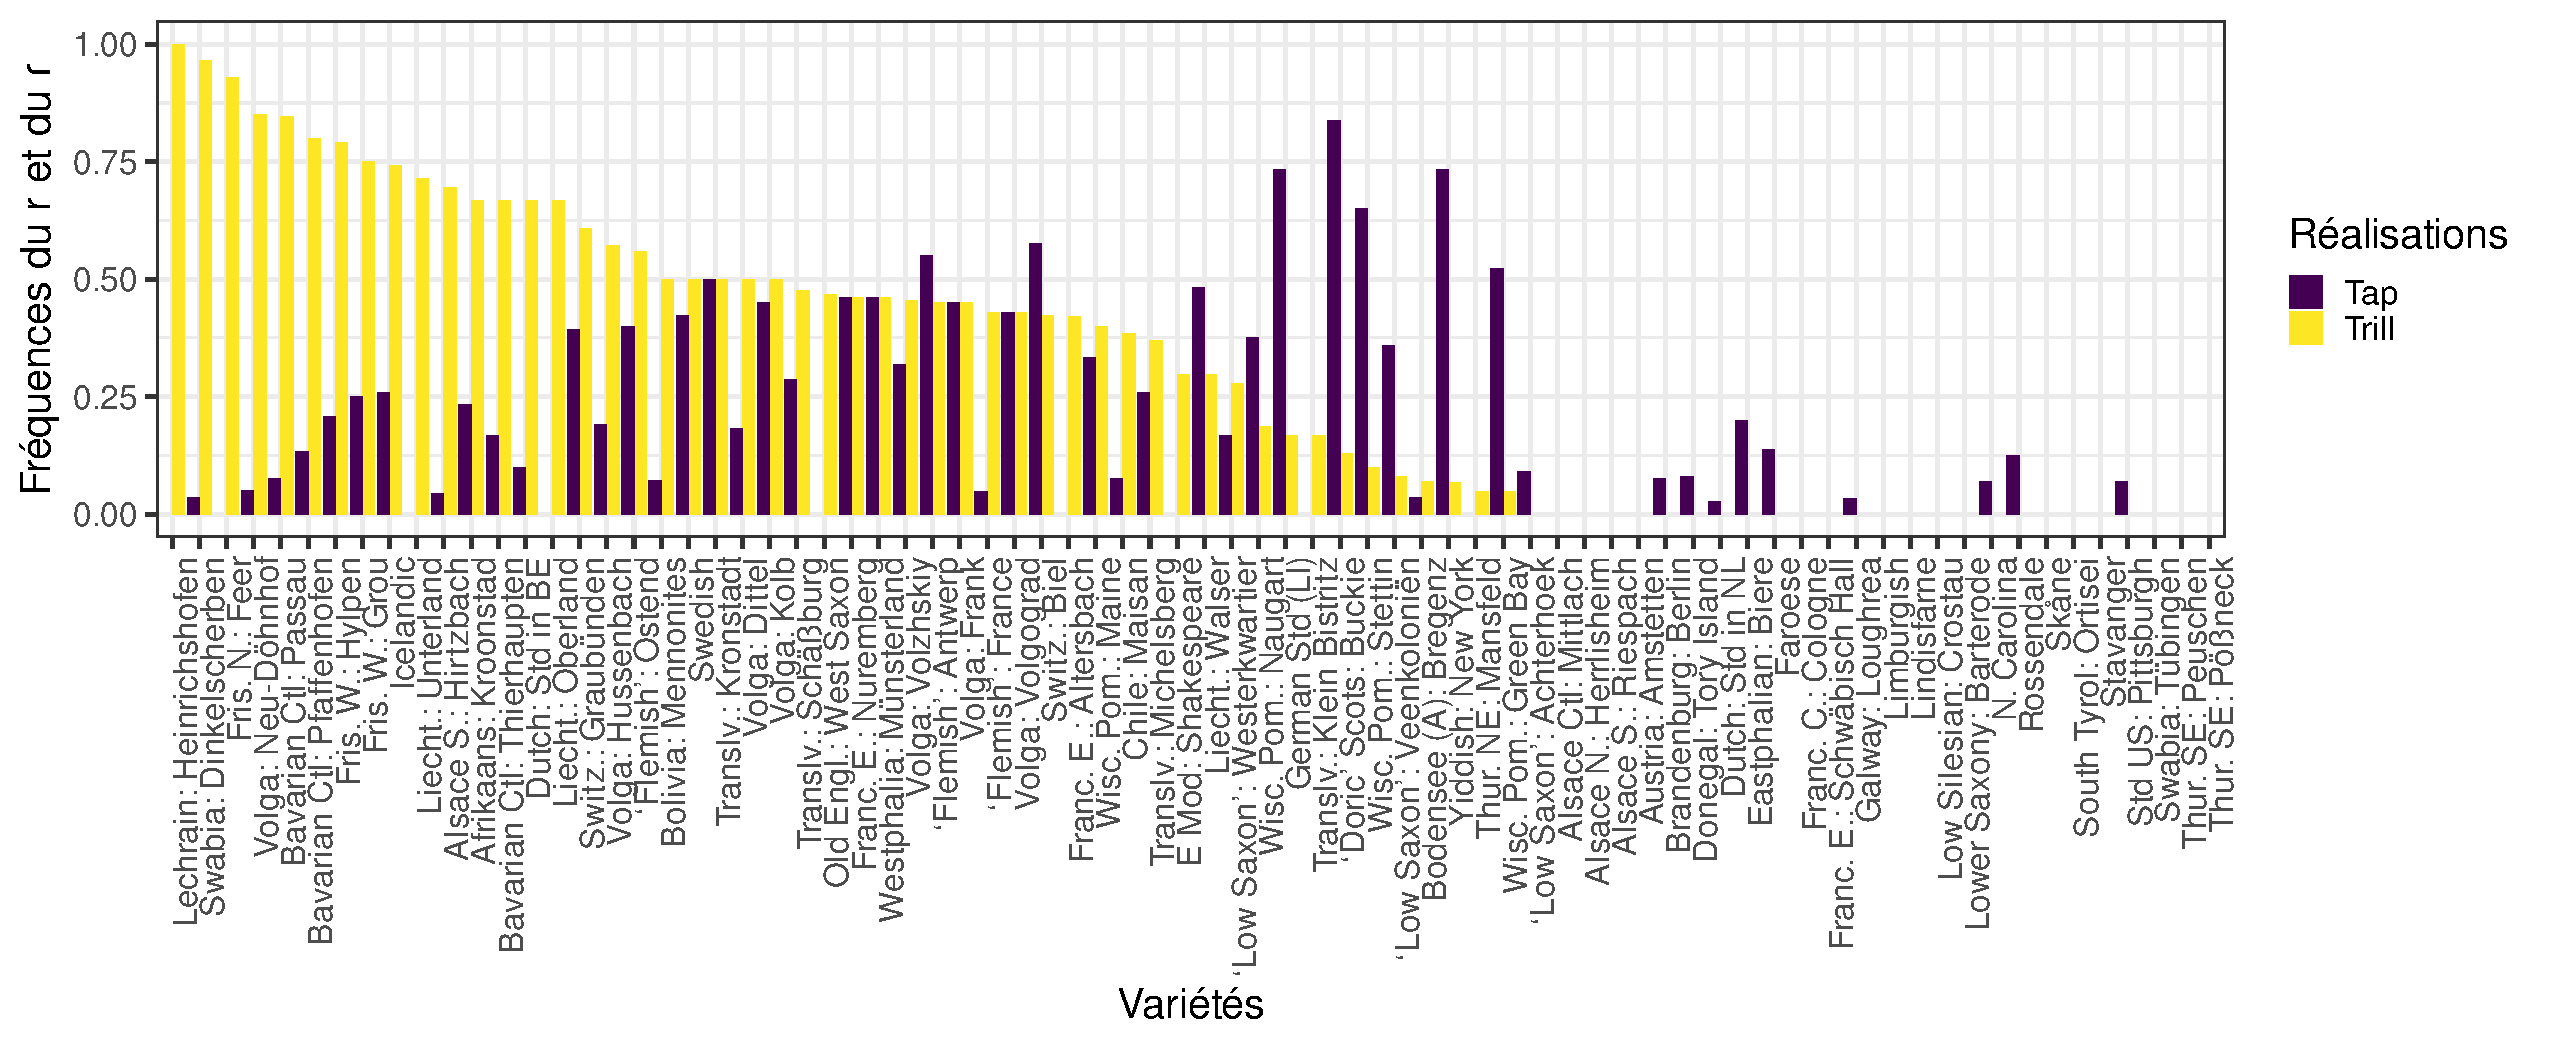
\includegraphics[width=1\linewidth]{substance/images/freq_trill_germanic2}
	\caption[Fréquences du trill et du tap dans les variétés germaniques]{Fréquences du trill et du tap dans les variétés germaniques. Seules les variétés où au moins un tiers des transcriptions ont été faites sont incluses. Les langues reconstruites ont été exclues.}
	\label{fig:freqtrillgermanic}
\end{figure}

La \autoref{fig:productiongermanic3viridis} présente de nombreuses variétés transcrites exclusivement avec un trill. Il s'agit de variétés reconstruites pour la plupart telles que le proto-germanique, le vieux frison, le néerlandais moyen, le vieux bas allemand, le vieux haut allemand, le  vieil islandais, le gothique.
On retrouve également le suédois parlé à \href{https://soundcomparisons.com/#/en/Germanic/language/Gmc_N_Swe_Fin_Ostrobothnia_Kronoby_Dl}{Kronoby en Ostrobothnie} et le \href{https://soundcomparisons.com/#/en/Germanic/language/Gmc_N_Swe_Fin_Ostrobothnia_Kronoby_Dl}{frison de l'est parlé à Schäddel}.
Pour le bavarois central de Bodenmais, les rhotiques ont été transcrites avec la voyelle pré-ouverte centrale [ɐ], non prise en compte dans notre analyse, biaisant les résultats en faveur d'une fréquence plus importante du trill.
Enfin, on a aussi le cas du \href{https://soundcomparisons.com/#/en/Germanic/language/Gmc_W_GHgh_Alm_Lech_Heinrichshofen_Dl}{haut allemand parlé à Heinrichshofen en Lechrain}. Il semblerait que des taps soient également présents dans ces variétés où le \textit{r} est majoritairement utilisé pour les transcriptions, et ce après vérification des enregistrements sonores avec Praat (nous avons uniquement vérifié les diminutions de l'intensité) mais sans pousser l'analyse acoustique comme dans le \autoref{chap:acoustics}.\\

Dans de nombreux cas (n = 24), lorsque le \textit{r} n'est pas le seul allophone, il représente plus de la moitié des allophones. Pour certains cas, lorsque le \textit{r} n'est pas l'allophone majoritaire mais que sa fréquence est supérieure à celle du tap, nous proposons deux hypothèses. D'un côté, il est possible que la tâche d'élicitation par mot a rendu plus favorable la production de trill. D'un autre côté, la transcription des variétés germaniques est plus large que celles des variétés romanes et slaves, en partie à cause du nombre important de collaborateurs et collaboratrices impliqués. Ces transcriptions plus larges favorisent l'usage du r.\\

En figure \ref{fig:freqtrillgermanic}, on observe que la fréquence maximale pour le trill est de 1 pour le \href{https://soundcomparisons.com/#/en/Germanic/language/Gmc_W_GHgh_Alm_Lech_Heinrichshofen_Dl}{haut allemand parlé à Heinrichshofen en Lechrain} (précédement mentionné).
En supprimant les variétés sans aucun trill, la moyenne de la fréquence du trill est à 0,48, sa médiane à 0,47 et son écart inter-quartile de 0,35.
Pour le tap, dans ces mêmes variétés avec des trills, sa fréquence moyenne est à 0,27, sa fréquence médiane est à 0,24 et son écart inter-quartile est de 0,40.\\

Au vu des résultats liés à ces transcriptions considérées comme plus larges, nous pouvons nous demander si des transcriptions plus larges ne sont pas synonymes d'une moyenne plus importante de \textit{r} dans les transcriptions. Cette hypothèse est soutenue par les résultats que nous avons obtenus dans le \autoref{chap:jipa} où nous trouvions plus de \textit{r} dans les transcriptions larges que dans les transcriptions étroites. Inversement, nous avions, en comparaison, plus de \textit{ɾ} dans les transcriptions étroites que dans les transcriptions larges. Il faut donc être précautionneux avec les \textit{r} dans les transcriptions, et en particulier les transcriptions larges. \\

Les différentes études nous donnent un résultat important : une variation quasi-inexistante dans les reconstructions phonétiques des rhotiques. Les langues historiques / proto-langues sont généralement caractérisées par des transcriptions pouvant être qualifiées de larges, et des inventaires de sons avec presque uniquement le symbole \textit{r} \parencite{marsicoBDPROTODatabasePhonological2018}.

\section{Etude de cas 4 : le cas du mapudungun \parencite{aninao_sound_2019}}

Nous avons fait le choix de ne pas inclure les résultats des transcriptions du mapudungun et de ses variétés/accents, transcrites dans la deuxième étude de cas, avec les langues romanes et slaves, bien qu'elles soient considérées comme étroites par \textcite{heggartySoundComparisonsNew2019} (p. 282). En effet, contrairement aux autres études, le mapudungun concerne une langue (et pas un groupe de langues) parlée dans plusieurs lieux géographiques. La langue appartient à la famille des langues araucaniennes \glotto{arau1255}.

\subsection{Description du mapudungun} \label{subsec:mapuche}

Le mapudungun est une langue parlée par quelques 152000 locuteurs au Chili et en Argentine, et répartie en plusieurs dialectes qui tendent à être \textg{abandonnés} en faveur de l'espagnol. \parencite{sadowskyMapudungun2013}. Les principales différences entre les dialectes proviennent de la phonétique \parencite{smeetsGrammarMapuche2008} (p. 11). L'\textit{Illustration of the IPA} du mapudungun se base sur des locuteurs/trices issu.e.s d'un sous-groupe du dialecte V (groupe central du mapudungun) ayant appris l'espagnol comme langue secondaire en moyenne vers 9 ans.
Dans son tableau consonantique, on retrouve la fricative voisée rétroflexe /ʐ/ qui peut se réaliser comme une fricative [ʐ ʂ], ou une approximante [ɻ] ou rétroflexe latérale [ɭ]. \textit{ʐ} est le symbole choisi pour représenter le phonème rhotique parce qu'il s'agit du variant prédominant dans l'échantillon des auteurs.
\textcite{smeetsGrammarMapuche2008} considère la phonétique et la phonologie du mapudungun \textg{plutôt simple} avec une glide rétroflexe \textit{r} avec peu de friction [ɹ̣] (soit en API [ɻ]). Dans les emprunts, il est considéré que les \textit{r} et \textit{rr} de l'espagnol sont remplacés par une approximante rétroflexe. Le \textit{r}, chez certains locuteurs, peut alterner avec đ, généralement produit comme [θ], s, généralement produit comme [s], sh, généralement produit comme [š] (soit en API [ɕ] ou [ʃ]), y, généralement produit comme [y] (soit en API [j]) et q (la glide vélaire soit probablement [ɣ̞] ou [w] en API).
\textcite{croeseEstudioDialectologicoMapuche1980} fait état de deux familles de phonèmes, ceux stables et ne présentant pas de variation interdialectale, et ceux instables caractérisés par leur fluctuation interdialectale (p. 12). Le /ṛ/ est considéré comme un phonème instable.\\


C'est parce que dans les transcriptions orthographiques on retrouve le <r> pour le /ʐ/, que nous avons décidé d'inclure le mapudungun à notre analyse des rhotiques.\\
Les transcriptions ont été faites par \href{https://sadowsky.cl/}{Scott Sadowsky}. Sa \href{http://repositorio.udec.cl/xmlui/handle/11594/4338}{thèse} \parencite{sadowskyNaturalezaFoneticaEstratificacion2012} en sociophonétique traite des allophones vocaliques dans une variété de l'espagnol du Chili, et on retrouve dans ses recherches en sociophonétique des descriptions précises du /r/ et du /ɾ/ en espagnol du Chili \parencite{sadowskyVariacionSociofoneticaConsonantes2015}.

\subsection{Résultats de la caractérisation de la rhotique en mapudungun}

\begin{figure}
	\centering
	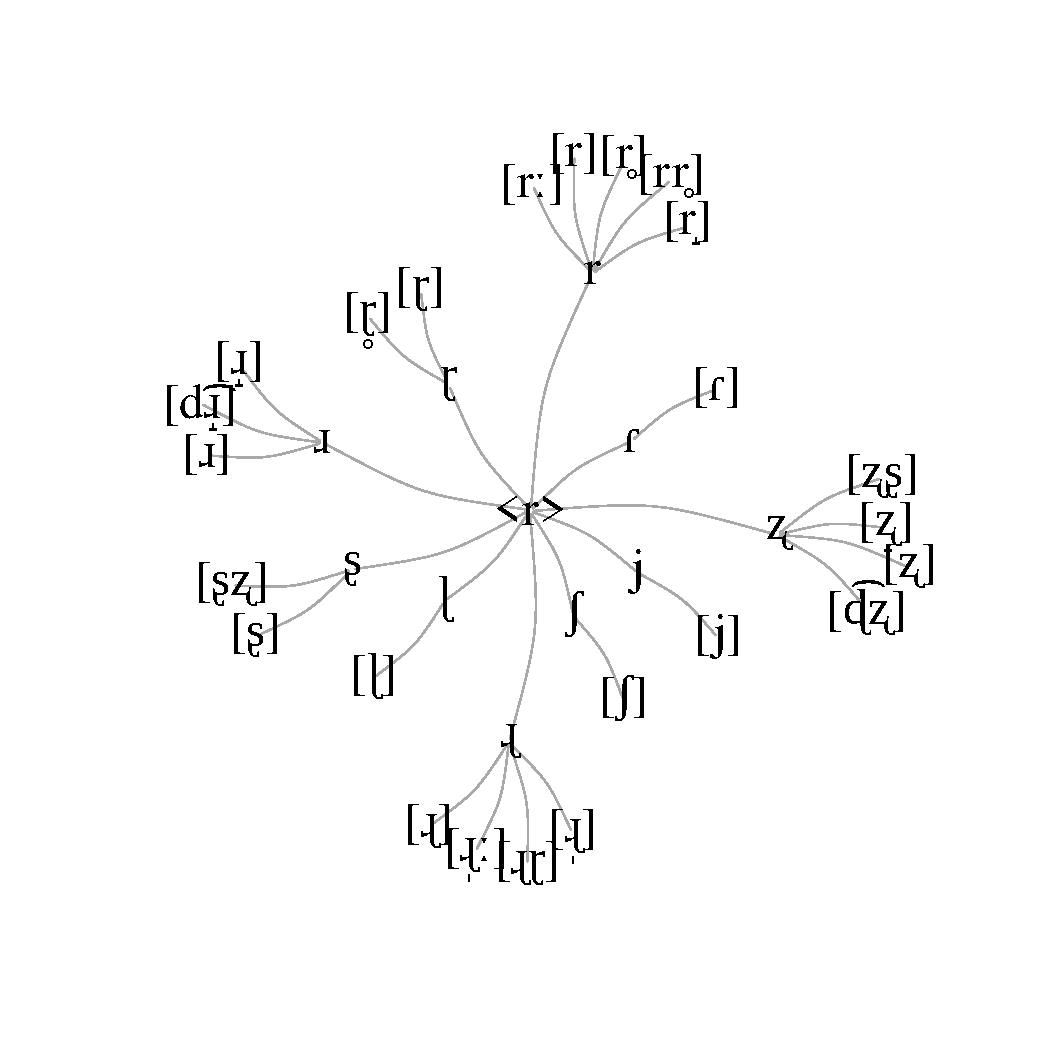
\includegraphics[width=0.7\linewidth]{substance/images/mapudungung_rhotics}
	\caption[Graphe des différentes réalisations de la rhotique dans les variétés mapudungun]{Graphe des différentes réalisations de la rhotique dans les variétés mapudungun à partir des données de Sound Comparisons. Le graphe est obtenu avec le package \texttt{igraph} \parencite{csardiIgraphSoftwarePackage2006}.}
	\label{fig:mapudungungrhotics}
\end{figure}

La figure \ref{fig:mapudungungrhotics}, obtenue à partir des données de Sound Comparisons, nous permet de  montrer que dix caractères forment le niveau d'analyse intermédiaire pour le mapudungun. Au total, il y a 24 réalisations possibles pour les différents cognats pris en compte. Nous avons regardé les transcriptions du <r> indépendamment de la position dans le mot (ce que nous n'avions pas fait pour les différentes variétés d'Europe).\\

Le <r> en mapudungun n'est jamais postérieur, il varie entre un lieu d'articulation alvéolaire, post-alvéolaire, rétroflexe et palatale. Il peut être produit comme un trill, un tap, une fricative ou comme une approximante (latérale ou non).
En moyenne, chaque caractère intermédiaire possède environ 2,4 réalisations.\\

\begin{figure}
	\centering
	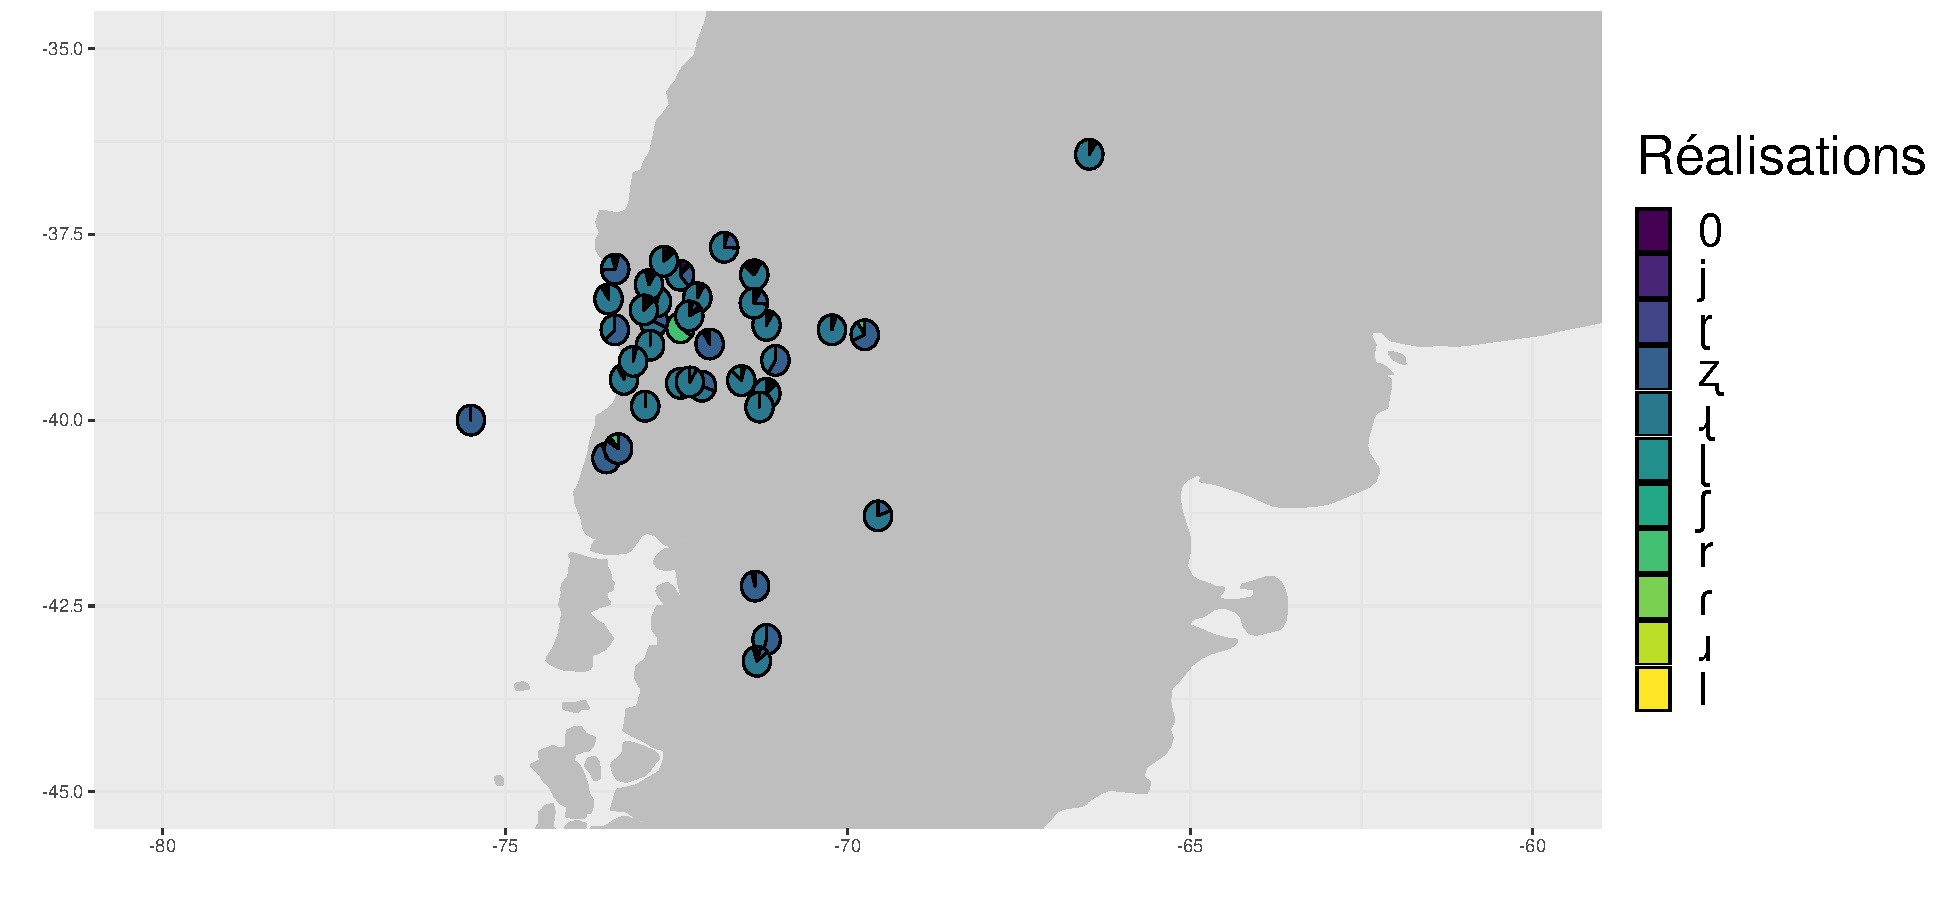
\includegraphics[width=1\linewidth]{substance/images/productionmapudungun_1_viridis}
	\caption[Distribution des différentes réalisations dans les variétés mapudungun]{Distribution des différentes réalisations dans les variétés mapudungun étudiées.}
	\label{fig:productionmapudungun1viridis}
\end{figure}

La variation transcrite par Scott Sadowsky se concentre à l'avant de la cavité orale, avec principalement des productions rétroflexes ʐ et ɻ (Figure \ref{fig:productionmapudungun1viridis}).\\

\begin{figure}
	\centering
	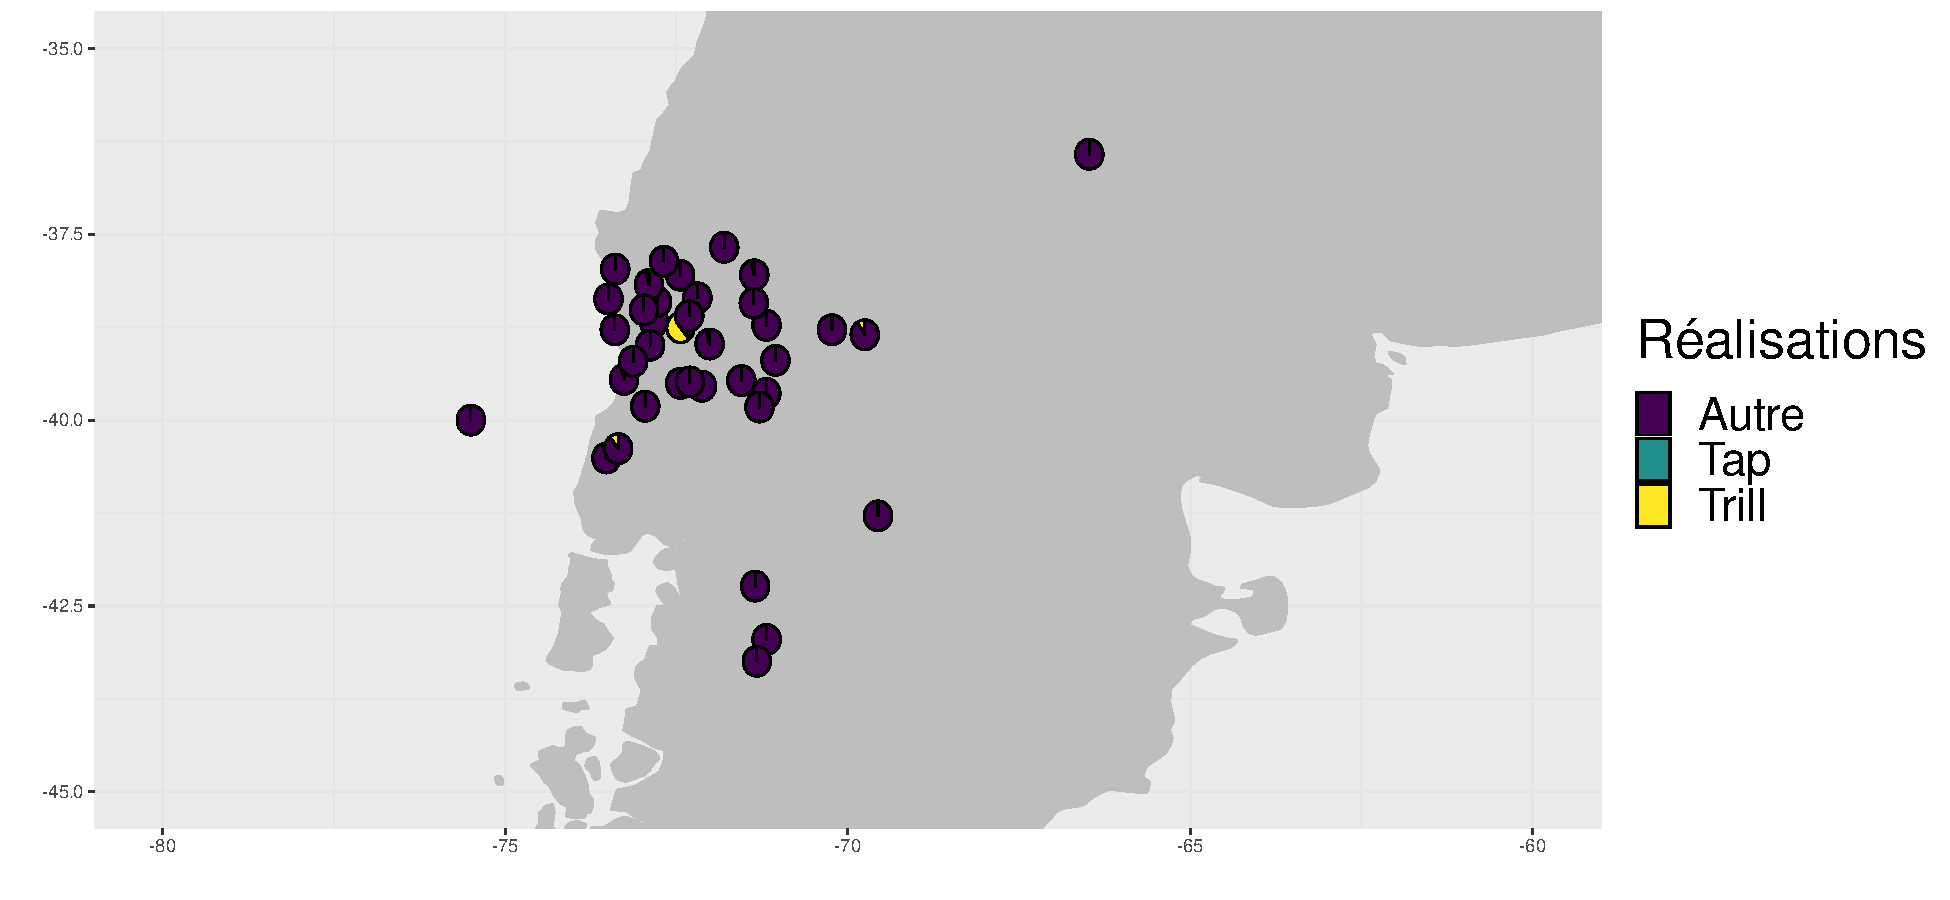
\includegraphics[width=1\linewidth]{substance/images/productionmapudungun_3_viridis}
	\caption[Distribution des différentes réalisations dans les variétés mapudungun pour le trill et tap]{Distribution des différentes réalisations dans les variétés mapudungun étudiées en ne s'intéressant qu'à la dichotomie entre trill et tap (et les autres segments).}
	\label{fig:productionmapudungun3viridis}
\end{figure}

\begin{figure}
	\centering
	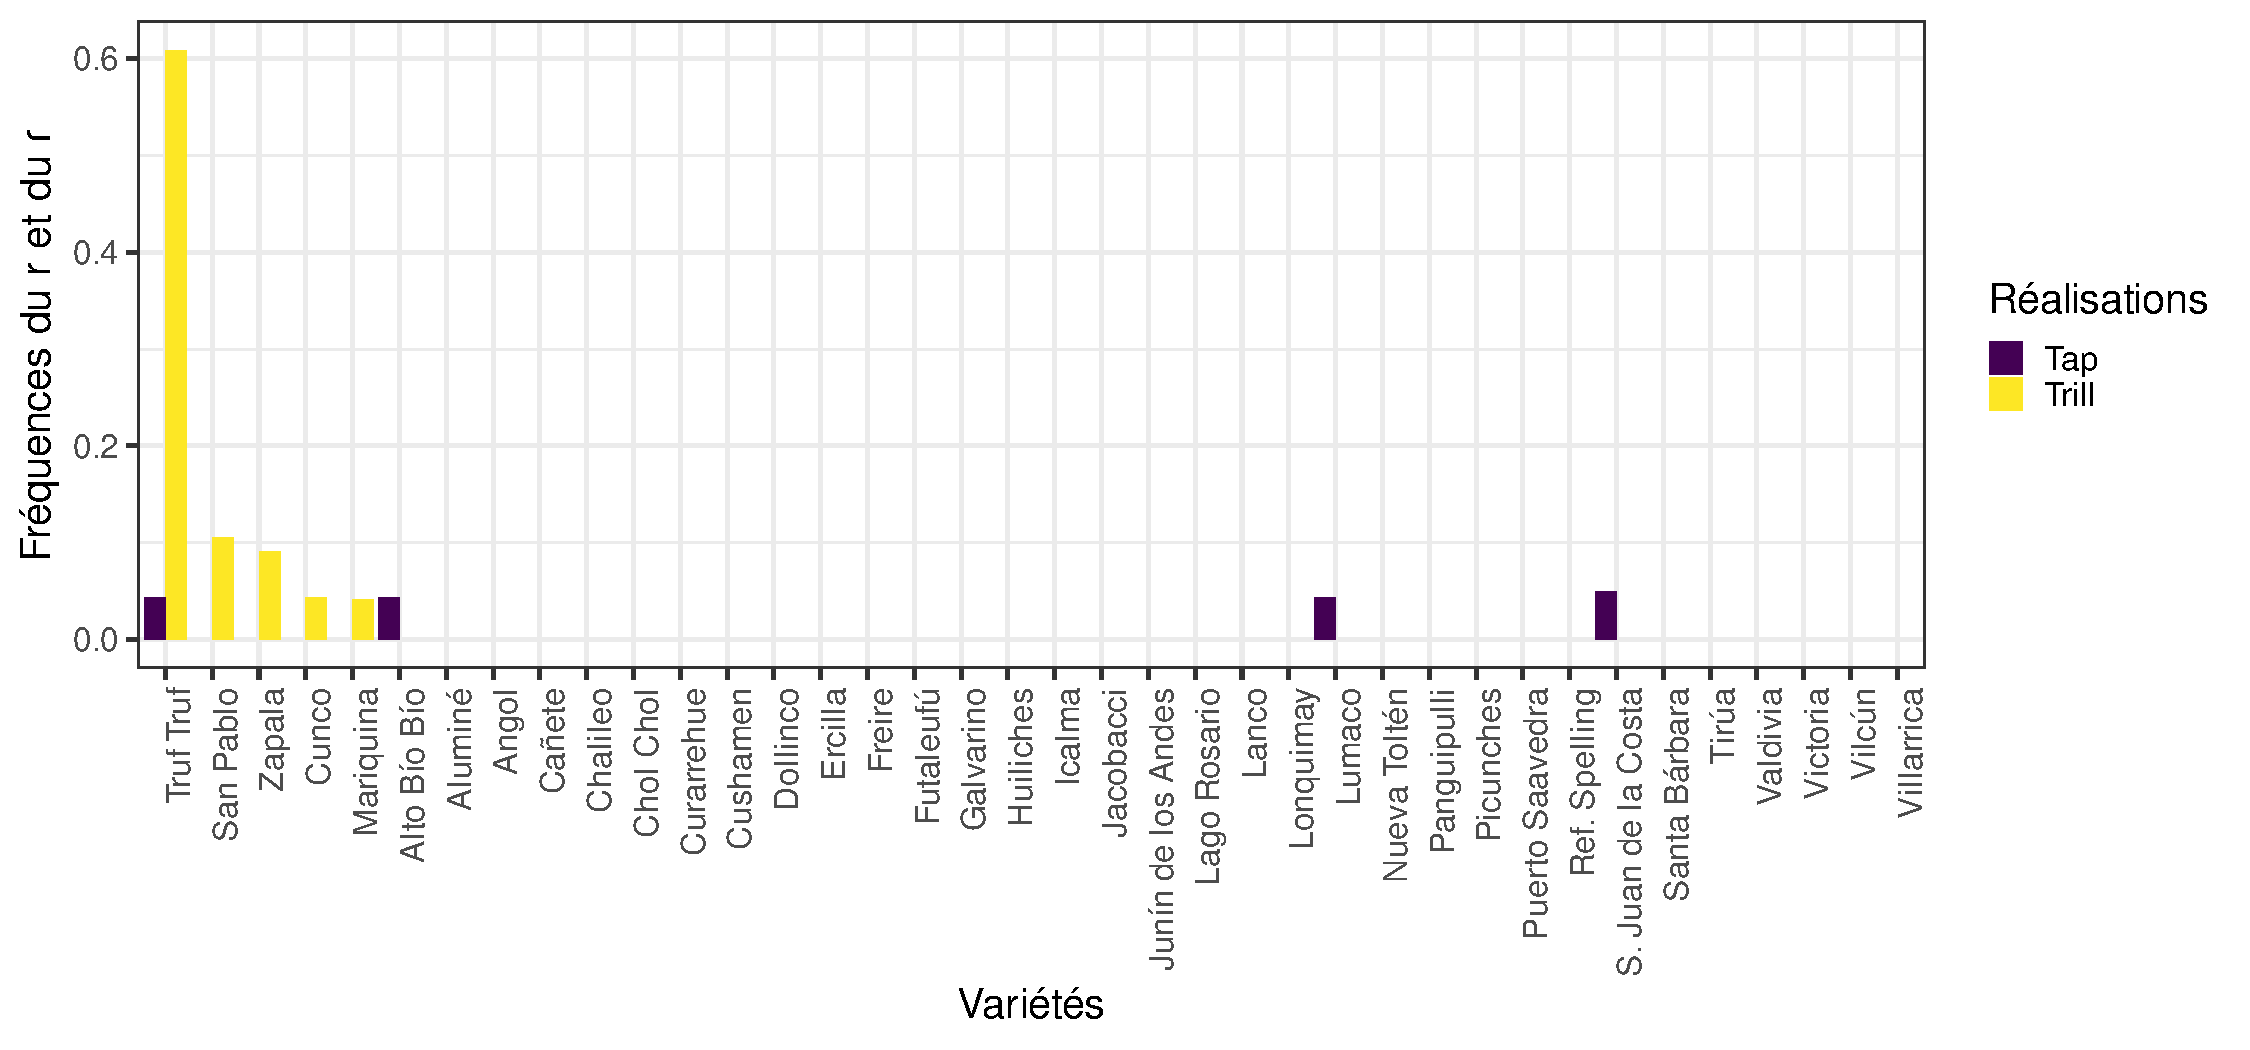
\includegraphics[width=1\linewidth]{substance/images/freq_trill_mapudungun2}
	\caption[Fréquences du trill et du tap dans les variétés mapudungun]{Fréquences du trill et du tap dans les variétés mapudungun. Seules les variétés où au moins 1/3 des transcriptions ont été faites sont incluses. Les langues reconstruites ont été exclues.}
	\label{fig:freqtrillmapudungun}
\end{figure}


\begin{table}
	\centering
	\resizebox{\linewidth}{!}{
	%\csvautobooktabular{substance/tables/production_classical_latin.csv}
	\csvautobooktabular{substance/tables/productions_trill_mapudungun.csv}}
	\caption[Transcriptions de certains cognats avec un \textrm{[r]} dans Sound Comparisons pour les variétés du mapudungun]{Transcriptions de certains cognats avec un [r] dans Sound Comparisons pour les variétés du mapudungun.}
	\label{tab:productiontrill_mapudungun}
\end{table}

Nous souhaitons mettre en avant la présence de trills et de taps dans les transcriptions. Sur les différentes variétés transcrites, nous ne retrouvons des trills que dans cinq d'entre elles (\href{https://soundcomparisons.com/#/en/Mapudungun/language/Mpg_Chl_Rgn9_TrufTruf_Danquilco}{Truf Truf}, \href{https://soundcomparisons.com/#/en/Mapudungun/language/Mpg_Chl_Rgn10_SanPablo_Quilacahuin}{San Pablo}, \href{https://soundcomparisons.com/#/en/Mapudungun/language/Mpg_Arg_Nqn_Zapala_RamonCastro}{Zapala}, \href{https://soundcomparisons.com/#/en/Mapudungun/language/Mpg_Chl_Rgn9_Cunco_Huerere}{Cunco}, \href{https://soundcomparisons.com/#/en/Mapudungun/language/Mpg_Chl_Rgn14_SanJoseMariquina_Maiquillahue}{Mariquina}).
La \autoref{fig:productionmapudungun3viridis} illustre bien la paucité du trill en mapudungun. Contrairement à nos études précédentes des données de Sound Comparisons, nous observons que la transcription des taps
ne correspond pas forcément aux variétés qui présentent un trill. Seulement une variété a été transcrite avec des trills et des taps.\\

En \autoref{fig:freqtrillmapudungun}, on observe que la fréquence maximale pour le trill est de 0,61 pour le \href{https://soundcomparisons.com/#/en/Mapudungun/language/Mpg_Chl_Rgn9_TrufTruf_Danquilco}{Truf Truf}.
En supprimant les variétés sans aucun trill, la moyenne de la fréquence du trill est à 0,18, sa médiane à 0,09 et son écart inter-quartile de 0,06.
Pour le tap, dans les variétés où on a des trills, sa fréquence moyenne est à 0,01, sa fréquence médiane est à 0 et son écart inter-quartile est de 0.
Si on s'intéresse aux transcriptions des différents mots avec un trill (\autoref{tab:productiontrill_mapudungun}), on remarque que le [r] est présent en attaque de syllabe mais peut se retrouver en coda. Il se trouve en syllabe accentuée mais aussi en syllabe non-accentuée.\\

Pourquoi retrouve-t-on des trills dans cinq variétés ?
Une des hypothèses est l'influence que l'espagnol a sur les locuteurs et locutrices du mapudungun. Les locuteurs et locutrices sont bilingues. Il n'est pas improbable que les [r] soient dus à l'influence du [r] espagnol. Pourtant, il faut rappeler que le /r/ en espagnol du Chili est aussi variable dans ses allophones et que certains allophones sont même stigmatisés. \textcite{sadowskyVariacionSociofoneticaConsonantes2015} résume que le [r] est principalement utilisé par les personnes nées après 1990. Le variant [ɹ], non stigmatisé, est utilisé par  les personnes nées avant 1990. Les allophones stigmatisés se retrouvent dans les classes basses et moyennes-basses et sont caractérisés par plus de friction. \citeauthor{sadowskyVariacionSociofoneticaConsonantes2015} explique l'existence d'une possible pression extérieure venant des moyens de communication pour la production des /r/ en [r] dans la jeune génération. Cette exposition massive joue selon lui un rôle dans ces productions (p. 85).
Et bien que les enregistrements sonores des locuteurs et locutrices permettent de supposer (sans aucune exactitude) leur naissance avant les années 1990, nous pouvons faire l'hypothèse que ces cinq locuteurs et locutrices ont été influencés eux aussi par ces moyens de communication.

%\subsubsection{Le cas des variétés des variétés du Quechua et du Vanuatu et de Papouasie de l'ouest}

\section{Discussion}

Dans ce chapitre, nous avons utilisé les données qui provenaient de Sound Comparisons, un projet collaboratif. Nous avons utilisé cinq études du projet pour proposer quatre études de cas. Nous avons analysé les transcriptions de différents cognats contenant une rhotique dans le but d'établir des inventaires des symboles utilisés que nous avons représentés sous la forme de graphes. Les réalisations qui peuvent être inférées des rhotiques sont multiples, et dépendent du style de transcription utilisé.
Les rhotiques varient autant dans les transcriptions étroites que larges, avec diverses réalisations. En effet, on retrouve différents lieux d'articulation mais aussi manières d'articulation.
Cependant, nous retrouvons des différences importantes pour l'étude du trill.
Les transcriptions larges, ainsi que les transcriptions des langues historiques ou proto-langues, ont tendance à plus utiliser le symbole \textg{r}.\\

Il ressort de nos analyses que lorsque les transcriptions sont étroites, le tap est le plus fréquent, et que pour les langues indo-européennes il ne peut pas y avoir de trill sans tap. Cela ne semble pas être entièrement le cas pour le mapudungun, dont le trill n'est pas natif. Nous pouvons nous demander si ce serait le cas pour d'autres familles de langues parlées dans d'autres régions du monde.\\

Finalement, avec ce chapitre nous avons aussi souhaité mettre en avant le travail des transcripteur/euses qui n'est pas sans difficultés. Transcrire implique d'avoir une vision globale de ce qui est productible mais aussi des symboles qui peuvent être associés. Ainsi, l'expérience en transcription, et l'intérêt pour la variation sont importants pour les études sur les rhotiques.